\documentclass[12pt]{article}

\usepackage{mypackages}
\usepackage{mycommands}
\usepackage{myenv}

\newtheorem{theorem}{Theorem}

\graphicspath{{figures/}}
% Shared drawing conventions. All geometry is schematic unless stated otherwise.
\definecolor{objectblue}{RGB}{36,79,116}
\definecolor{motionteal}{RGB}{0,113,119}
\definecolor{forceorange}{RGB}{170,76,20}
\tikzset{
  paperfigure/.style={font=\footnotesize,>=Stealth,line width=.65pt},
  object/.style={draw=objectblue,fill=objectblue!7},
  feature/.style={draw=black!65,fill=black!13},
  motion/.style={draw=motionteal,->},
  force/.style={draw=forceorange,->,line width=.9pt},
  guide/.style={draw=black!45,densely dashed,line width=.45pt},
  paneltitle/.style={anchor=west,font=\small\bfseries},
  callout/.style={fill=white,inner sep=2pt,font=\footnotesize},
}


\title{Shift, Then Turn: Planar In-Grasp Manipulation with Two Passive Rods}
\author{Pierre-Olivier Bolduc, Clément Gosselin}
\date{October 2026}

\begin{document}

\maketitle

\begin{abstract}
Parallel grippers are reliable and inexpensive, but once they pinch an object they cannot change its pose within the grasp. Rather than adding sensing, finger actuation, or contact-rich planning, we add passive geometry to the robot's workspace, and we show that this geometry can be designed in closed form. The design starts from what passive contacts can and cannot do: they cannot determine a motion that both slides and turns the object in the grip, so a planar change of grasp is executed as a shift, during which the tool holds the object while the gripper slides along it, followed by a turn, during which the gripper orbits one contact while the grasp holds. Two rods spinning freely on bearings provide both motions. Two rods are the fewest that hold an arbitrary shift; one of them then guides the turn, and the other separates by itself. The rod placement is a projection at one vertex of a convex or nonconvex polygonal outline, the gripper path is a segment followed by a circular arc, and a single quadratic equation tells whether an installed pair can serve a request. No friction coefficient or grip-force value enters the design, no sensing is used during the manipulation motion, and because the rods spin freely, grasp slip during the turn is predicted from the pad size and the lever arm alone. Hardware turns on a Kinova Jaco reached mean absolute errors of $3.6^{\circ}$--$7.5^{\circ}$; in simulation, complete sequences ended within $1.6^{\circ}$ and 0.44 mm of the request, and the measured tilt, slip, and separation agreed with the closed-form predictions.
\end{abstract}

\section{Introduction}
\label{sec:intro}

Most industrial robots use simple end-effectors, such as parallel grippers, because they are reliable, inexpensive, and easy to control. They suffice for pick-and-place, but once an object is grasped they offer little control over its pose within the grasp. That pose often matters. A part picked from a bin wherever it was easiest to grasp must frequently be presented to a fixture, a machine, or an assembly in one particular grasp; today this requires a regrasp station, a dedicated jig, or a more dexterous hand. A gripper that could adjust its grasp in place would remove that step, and it would also relax the constraints on the initial grasp.

People face the same limitation with one hand and overcome it with a second hand, even one that does very little. Holding an object still while the fingers slide along it, or giving it a point to pivot about, is often enough. A passive tool in the workspace can play this role: contact with the tool holds or guides the object while the robot moves the gripper. This makes the workspace a design variable for in-hand manipulation. The question is then what geometry to add, where to place it, and how to move the robot so that a desired change of grasp follows from those contacts. Our thesis is that this question has a closed-form answer. Instead of giving a simple gripper more sensing, actuation, or planning, we give its workspace the geometry it is missing, and we show that this geometry can be designed in closed form.

External assistance is an established route to dexterity with simple grippers. Extrinsic dexterity uses forces from gravity, inertia, and environmental contacts to change an object's pose within the grasp \cite{dafle2014extrinsic}. Prehensile pushing constructs such changes by pressing a grasped object against fixed features in the environment \cite{chavan2015prehensile,chavan2018stable}; sampling-based planners and motion cones chain these pushes into regrasps, including motions that combine sliding and turning, by modelling the frictional contacts between gripper, object, and pusher \cite{chavan2017sampling,chavan2020planar}. Fixtureless fixturing pushes the object against an environmental feature that holds it still while the fingers slide over it \cite{chavan2018fixtureless}, the closest precedent for the shift studied here. Pivoting against the environment and shared grasping reorient objects through contact with a support \cite{hou2019reorienting,hou2020manipulation}, inertial loads can drive in-grasp sliding \cite{shi2017dynamic}, and visual and tactile feedback can regulate pivoting \cite{karayiannidis2016adaptive,toskov2023hand,kim2024texterity}. These methods establish that interaction with the environment extends a gripper's capabilities. They take the environment as given, however, and obtain the motion from friction coefficients, grip-force values, numerical planning, or feedback (\tabref{tab:positioning}).

\label{sec:related}
Designing the constraints themselves has a long history. Passive fences orient parts, modular fixtures constrain them through deliberately chosen contact geometry, and sensorless orienting uses geometric contact sequences \cite{wiegley1997complete,brost1996complete,goldberg1993orienting,asada1985fixturing}; their objective is a final part pose, not a change of pose while the part remains in a gripper. Effector form design derives a finger's shape from the motion it must produce \cite{rodriguez2013effector}, and bearings or passive rollers in the fingers make pivoting and sliding within the grasp mechanically easier \cite{carlisle1994pivoting,fisk2026rollers}; these approaches modify the gripper, whereas we leave it unchanged and design a fixture in the workspace. Open-loop pivoting shows that a simple gripper can reorient an object without feedback \cite{holladay2015general,cruciani2017hand}. Our earlier assistive tool used two planes with their angle selected through simulation \cite{bolduc2023inhand}; here the tool's geometry and placement follow from analysis instead. The analysis draws on classical planar contact mechanics: instantaneous rotation centres on contact normals \cite{mason2001mechanics}, first- and second-order contact constraints \cite{ohwovoriole1981extension,rimon1998mobility}, the mechanics of pushing \cite{mason1986mechanics,peshkin1988planning,lynch1996stable}, and limit surfaces for sliding contact patches \cite{goyal1991planar,howe1996practical,xydas1999modeling}. These ingredients are classical; what has been missing is their use as a design method for workspace geometry. Among the approaches compared in \tabref{tab:positioning}, ours is the only one that designs the workspace and changes the grasp in place, and the only one in which no friction coefficient, grip-force value, numerical planner, or feedback enters the manipulation motion.

\begin{table}[htbp]
    \centering
    \footnotesize
    \renewcommand{\arraystretch}{1.15}
    \setlength{\tabcolsep}{4pt}
    \begin{tabular}{>{\raggedright\arraybackslash}p{3.3cm}*{5}{>{\centering\arraybackslash}p{1.62cm}}>{\centering\arraybackslash}p{2.0cm}}
        \hline
        Approach & Same gripper & Workspace designed & Grasp changed in place & Friction or force in the plan & Feedback in motion & Motion computed by \\
        \hline
        Fences, modular fixtures, sensorless orienting \cite{wiegley1997complete,brost1996complete,goldberg1993orienting} & yes & yes & no & -- & no & complete search \\
        Prehensile pushing, motion cones, fixtureless fixturing \cite{chavan2015prehensile,chavan2017sampling,chavan2018fixtureless,chavan2020planar} & yes & no & yes & yes & no & sampling, optimization \\
        Pivoting, shared grasping \cite{hou2019reorienting,hou2020manipulation} & yes & no & yes & yes & force control & contact-mode planning \\
        Feedback-regulated pivoting \cite{karayiannidis2016adaptive,toskov2023hand,kim2024texterity} & yes & no & yes & estimated & vision, touch & controller \\
        Rollers or bearings in the fingers \cite{carlisle1994pivoting,fisk2026rollers} & no & no & yes & varies & varies & varies \\
        \textbf{Two free rods (this work)} & \textbf{yes} & \textbf{yes} & \textbf{yes} & \textbf{no} & \textbf{no} & \textbf{closed form} \\
        \hline
    \end{tabular}
    \caption{What approaches to changing a grasp with a simple gripper require. ``Friction or force in the plan'': whether a friction coefficient or a grip-force value is needed to compute the motion. ``Feedback in motion'': sensing used while the object is being manipulated, not to locate it beforehand.}
    \label{tab:positioning}
\end{table}

The proposed tool consists of two rods that spin freely on bearings (\figref{fig:tworod}). The gripper pinches a planar object across its thickness and first brings it against both rods. During a shift, the rods hold the object still while the gripper slides along it. During a turn, the gripper orbits one rod and the object pivots within the grasp. The wrist orientation stays fixed during each manipulation motion. A requested planar displacement is decomposed into a shift followed by a turn; when both rods contact the same edge, the object is carried away and re-engaged before turning. The tool amounts to two pins on bearings: it leaves the gripper and its controller unchanged, and the manipulation motions themselves need no sensing.

The paper makes four contributions:
\begin{itemize}
    \item \emph{A design principle for passive in-grasp manipulation.} We show why passive contacts with a fixed wrist cannot uniquely determine simultaneous sliding and turning within the grasp. This motivates separating a planar change of grasp into a shift and a turn (Section~\ref{sec:design}).
    \item \emph{A minimal tool with a closed-form design.} We establish that two rods are the minimum needed to support an arbitrary shift in one motion, and show how the same pair supports a subsequent turn. We derive the rod placements, gripper paths, and conditions under which an installed pair can perform a requested change of grasp (Sections~\ref{sec:method}, \ref{sec:tworod}, and~\ref{sec:installation}).
    \item \emph{Motion computation without friction or force parameters.} The manipulation motions require neither friction coefficients nor grip-force values as planning inputs. Freely rotating rods also allow grasp slip during a turn to be predicted from the finger-pad size and the lever arm (Section~\ref{sec:turn}).
    \item \emph{Experimental and simulation evidence.} We validate turns on hardware and evaluate shifts and complete shift--turn sequences in simulation, comparing the results with the analytical predictions (Section~\ref{sec:experiments}).
\end{itemize}

Execution assumes a known initial grasp pose and grip settings that retain the object while permitting the required sliding and pivoting; contact, grasp travel, clearance, and robot reach must also be checked. Hardware trials with a single rod demonstrate the turn in the vertex-contact case covered by the analysis, and shifts and complete sequences are tested in simulation.

\begin{figure}[htbp]
\centering
% Computed from the shift and turn constructions for a convex pentagon (mm, 1 mm = 0.05 cm):
% Delta = 80 deg, d = (6,18) mm, R = 5 mm, lambda = 34 mm. Written by python -m geometry; do not edit coordinates by hand.
\begin{tikzpicture}[paperfigure,
  gripbody/.style={fill=black!55,draw=black!80,line width=.4pt},
  grippad/.style={fill=black!75,draw=black},
  ghostobj/.style={draw=objectblue!60,densely dashed,fill=none,line width=.5pt}]
\newcommand{\gripper}[3]{%
  \begin{scope}[shift={(#1,#2)},#3]
    \fill[gripbody,rotate=30] (-3,0) rectangle (3,-24);
    \fill[grippad] (0,0) circle[radius=4];
    \fill[white] (0,0) circle[radius=1];
  \end{scope}}
\path[use as bounding box] (0,-0.10) rectangle (15.6,11.1);

\node[paneltitle] at (0,10.9) {(a) Engage};
\begin{scope}[shift={(4.084,9.114)},x=0.05cm,y=0.05cm]
\draw[ghostobj] (-28.26,-21.01) -- (35.74,-25.01) -- (51.74,-2.01) -- (23.74,17.99) -- (-34.26,8.99) -- cycle;
\draw[object] (-34.00,-17.00) -- (30.00,-21.00) -- (46.00,2.00) -- (18.00,22.00) -- (-40.00,13.00) -- cycle;
  \draw[feature] (-35.76,18.72) circle[radius=5]; \fill (-35.76,18.72) circle(.6pt);
  \draw[feature] (-43.12,3.09) circle[radius=5]; \fill (-43.12,3.09) circle(.6pt);
  \draw[motion,line width=.9pt] (30.00,-26.00) -- (20.16,-19.13);
  \gripper{0.00}{0.00}{}
  \node[anchor=south] at (-35.76,24.22) {$a$};
  \node[anchor=east] at (-48.62,3.09) {$b$};
\end{scope}
\node[paneltitle] at (8.0,10.9) {(b) Shift};
\begin{scope}[shift={(11.898,9.071)},x=0.05cm,y=0.05cm]
\draw[object] (-34.00,-17.00) -- (30.00,-21.00) -- (46.00,2.00) -- (18.00,22.00) -- (-40.00,13.00) -- cycle;
  \draw[guide] (-39.57,5.87) -- (25.72,-3.81);
  \node[anchor=south west,inner sep=1pt,text=black!60] at (11.72,-2.31) {grasp line};
  \draw[feature] (-35.76,18.72) circle[radius=5]; \fill (-35.76,18.72) circle(.6pt);
  \draw[feature] (-43.12,3.09) circle[radius=5]; \fill (-43.12,3.09) circle(.6pt);
  \draw[guide] (-35.00,13.78) -- (-33.63,4.99);
  \draw[force] (-37.45,29.59) -- (-35.07,14.27);
  \draw[guide] (-38.21,4.07) -- (-33.63,4.99);
  \draw[force] (-53.90,0.93) -- (-38.70,3.97);
  \fill (-33.63,4.99) circle(1.2pt); \node[anchor=north west,inner sep=1pt] at (-32.83,4.19) {$\mathbf x$};
  \gripper{0.00}{0.00}{,opacity=.28}
  \draw[motion,line width=1pt] (-2.97,0.44) -- (-15.80,2.34);
  \node[anchor=south,inner sep=2pt] at (-9.38,3.39) {$-\mathbf d_0$};
  \gripper{-18.77}{2.78}{}
\end{scope}
\node[paneltitle] at (0,6.764132811653769) {(c) Turn};
\begin{scope}[shift={(4.278,1.647)},x=0.05cm,y=0.05cm]
\draw[ghostobj] (-34.00,-17.00) -- (30.00,-21.00) -- (46.00,2.00) -- (18.00,22.00) -- (-40.00,13.00) -- cycle;
\draw[object,fill opacity=.45,draw opacity=.45] (-11.45,-7.51) -- (40.14,30.56) -- (37.62,58.47) -- (3.31,55.79) -- (-35.33,11.61) -- cycle;
\draw[object] (-0.28,14.25) -- (14.77,76.58) -- (-5.10,96.33) -- (-29.66,72.23) -- (-30.87,13.55) -- cycle;
  \draw[feature] (-35.76,18.72) circle[radius=5]; \fill (-35.76,18.72) circle(.6pt);
  \draw[feature] (-43.12,3.09) circle[radius=5]; \fill (-43.12,3.09) circle(.6pt);
  \draw[motion,line width=1pt] (-18.77,2.78) arc[start angle=-43.156,end angle=36.844,radius=23.296];
  \gripper{-18.77}{2.78}{,opacity=.28}
  \gripper{-12.50}{17.43}{,opacity=.28}
  \gripper{-17.12}{32.69}{}
  \node[anchor=east] at (-41.26,21.72) {$a$};
  \node[anchor=east] at (-48.62,3.09) {$b$};
\end{scope}
\node[paneltitle] at (8.0,6.764132811653769) {(d) Result};
\begin{scope}[shift={(11.550,3.282)},x=0.05cm,y=0.05cm]
\draw[ghostobj] (-34.00,-17.00) -- (30.00,-21.00) -- (46.00,2.00) -- (18.00,22.00) -- (-40.00,13.00) -- cycle;
\draw[object] (16.84,-18.44) -- (31.89,43.90) -- (12.02,63.65) -- (-12.54,39.55) -- (-13.75,-19.13) -- cycle;
  \fill[objectblue] (6.00,18.00) circle(1.3pt);
  \draw[motion,line width=.9pt] (0,0) -- (5.52,16.56);
  \node[anchor=east,inner sep=2pt] at (3.30,9.90) {$\mathbf d$};
  \draw[motion,line width=.9pt] (26,-4) arc[start angle=-10,end angle=70,radius=26];
  \node[anchor=west] at (31,14) {$\Delta=80^\circ$};
  \gripper{0.00}{0.00}{}
\end{scope}
\draw[black!15] (7.8,-0.10) -- (7.8,11.0); \draw[black!15] (0,7.01) -- (15.6,7.01);
\end{tikzpicture}
\caption{Changing the grasp with two rods, using the constructions of Sections~\ref{sec:method} and~\ref{sec:turn}. (a)~The gripper brings the plate against two installed rods that spin freely on bearings. Dark disk: gripper pad; bar: wrist, whose orientation stays fixed throughout. (b)~The rod forces (orange) act along push lines meeting at $\mathbf x$ on the grasp line: the plate stays still while the gripper slides by $-\mathbf d_0$. (c)~The gripper orbits rod~$a$; the plate pivots within the grip, turns by $\Delta$, and separates from rod~$b$. (d)~In the gripper frame, the plate has turned by $\Delta=80^\circ$ and shifted by the requested $\mathbf d=\mathbf Q(\Delta)\mathbf d_0$. Teal arrows: gripper motion in (a--c), relative object displacement and rotation in (d); dashed outlines: initial poses.}
\label{fig:tworod}
\end{figure}

\section{Task and Design Requirements}
\label{sec:setting}

The task is to change an object's planar pose relative to a parallel gripper while retaining it in the grasp. The gripper pinches the object across its thickness, with gravity normal to the manipulation plane, so the object's weight acts along the pinch axis and does not enter the planar analysis. At engagement the gripper's world pose is $(\mathbf r^w_0,\psi_0)$; the wrist orientation $\psi_0$ is then held fixed. Vectors are expressed in the object frame, which coincides with the gripper frame at engagement, has its origin at the initial grasp, and moves with the object. A superscript $w$ marks the same vector in the world frame; for example, a rod centre is $\mathbf q$ in the object frame and $\mathbf q^w$ in the world frame. A request specifies the object's final pose relative to the gripper: a turn $\Delta$ and a displacement $\mathbf d$, with $\mathbf Q(\cdot)$ the planar rotation by a given angle. We take $\Delta\geq0$, a counterclockwise turn, without loss of generality: a clockwise turn is the mirror image of the same construction.

The object is rigid, with a polygonal outline $P$, convex or not, and a known initial grasp in its interior. Manipulation is quasi-static. The gripper touches the object through a pad centred on the grasp, and the grasp is usable while the pad's footprint lies inside $P$; these grasp positions form the usable grasp region. The grip must retain the object while permitting sliding and pivoting when the object is pressed against the tool. Planning uses no friction coefficient or grip-force value. The only friction model we invoke, in Section~\ref{sec:slip}, is the shape of the pad's limit surface, and the coefficient and force cancel from it.

The design objective is a passive workspace tool that enables both changes of position and changes of orientation without adding finger actuation or requiring wrist rotation during manipulation. Its geometry must supply the contact constraints, and its placement must admit robot access, usable grasp travel, and collision-free motion.

\section{Passive Contacts Require a Shift, Then a Turn}
\label{sec:design}

The tool must provide two capabilities: hold the object while the gripper slides, and guide a turn while the grasp point is retained. Rods provide localized contacts that can be positioned on different edges of the object. This section fixes the contact model and shows that a passive tool can determine these two motions only one at a time.

\subsection{Geometric contact model}
\label{sec:contact_model}

The outline $P$ is traversed counterclockwise, with vertices $\mathbf P_i$; edge $i$ runs from $\mathbf P_i$ to $\mathbf P_{i+1}$ and has outward unit normal $\mathbf n_i$. For a planar vector $\mathbf a$, $\mathbf a^\perp=\mathbf Q(\pi/2)\mathbf a$ is $\mathbf a$ turned by a quarter turn, and $\mathbf a\times\mathbf b=(\mathbf a^\perp)^T\mathbf b$. A rod has radius $R$ and a fixed axis normal to the manipulation plane. It touches $P$ at a point $\mathbf p$ with contact normal $\mathbf n$: the edge normal on an edge, or, at a convex vertex, any unit vector between the normals of its two edges. The rod centre satisfies
\begin{equation}
  \mathbf q=\mathbf p+R\mathbf n,\qquad \operatorname{dist}(\mathbf q,P)=R.
  \label{eq:rod_center}
\end{equation}
The distance check excludes penetration elsewhere. We also require each rod to touch $P$ at a single point, which excludes a rod wedged against two features at once and, together with the distance check, concavities narrower than the rod. Then $\operatorname{dist}(\cdot,P)$ is differentiable at $\mathbf q$ with unit gradient $\mathbf n$, for convex and nonconvex outlines alike. A rod spinning freely on its bearing exerts no tangential force, so its reaction acts along $-\mathbf n$ on the push line through $\mathbf p$ and $\mathbf q$. Its moment about the grasp, per unit force and positive counterclockwise, is the lever arm
\begin{equation}
  \ell=\mathbf p\times(-\mathbf n).
  \label{eq:edge_identity}
\end{equation}
A shift needs the rods' moments to cancel; a turn needs one rod with $\ell>0$.

\subsection{What passive contacts can prescribe}
\label{sec:separation}

A rod's surface moves only tangentially, whether the rod is fixed or spins on its bearing, so an engaged contact requires the object point at $\mathbf p$ not to move along $\mathbf n$. A small rotation of the object about some point moves $\mathbf p$ perpendicular to the line joining that point to $\mathbf p$, which has no component along $\mathbf n$ exactly when the point lies on the push line. Hence, if the object turns in the world about some point, the push line of every engaged contact passes through that point: the classical construction of instantaneous rotation centres from contact normals \cite{mason2001mechanics}. A rotation about that point neither enters nor leaves any contact. If the grasp point may also slide on the object, nothing else constrains the object's pose relative to the gripper, so the gripper path does not determine the turning angle. The motion is determined only in two cases: the object stays still in the world, giving a pure shift, or the grip holds the grasp point while a rod contact is maintained, giving a pure turn (Section~\ref{sec:turn}). A passive tool can therefore either hold the object while the grasp slides, or guide a rotation while the grasp holds, but not both at once. This does not prohibit combined motions obtained using additional mechanical information or feedback: motion cones, for instance, plan combined sliding and turning against fixed pushers from models of contact friction and grip force \cite{chavan2020planar}. It rules them out for a tool planned from geometry alone, and it is the price paid for a plan in which no friction coefficient or force value appears.

\subsection{Operating principle: hold, then guide}

In the shift mode, the object remains still in the world while the gripper translates along it. The grasp moves to a new point on the object, producing a relative displacement. In the turn mode, the grip holds that grasp point while the gripper follows an arc about one rod. The object pivots within the fixed-orientation grip, producing a relative rotation. We execute the shift first and the turn second, with the requested pose factored as
\begin{equation}
  \begin{bmatrix}\mathbf Q(\Delta)&\mathbf d\\\mathbf 0^T&1\end{bmatrix}
  =\begin{bmatrix}\mathbf Q(\Delta)&\mathbf 0\\\mathbf 0^T&1\end{bmatrix}
   \begin{bmatrix}\mathbf I&\mathbf d_0\\\mathbf 0^T&1\end{bmatrix},
  \qquad \mathbf d_0=\mathbf Q(\Delta)^T\mathbf d.
  \label{eq:factor}
\end{equation}
Thus the shift vector is $\mathbf d_0$, which the subsequent turn rotates into the requested final displacement $\mathbf d$. Section~\ref{sec:method} shows that holding an arbitrary shift requires two rods, Section~\ref{sec:turn} shows that a turn requires one, and Section~\ref{sec:tworod} shows how the same pair passes from the first mode to the second.

\section{Shift: Hold the Object with Two Rods}
\label{sec:method}
\label{sec:shift}

For a shift, the rods hold the object still while the gripper translates:
\begin{equation}
  \mathbf r^w(s)=\mathbf r^w_0-s\,\mathbf Q(\psi_0)\mathbf d_0,\qquad s\in[0,1].
  \label{eq:shift_path}
\end{equation}
The relative object displacement is then $\mathbf d_0$, and the grasp travels along the segment from $\mathbf 0$ to $-\mathbf d_0$ on the object, which must lie in the usable grasp region. For a nonzero shift, write $\hat{\mathbf d}_0=\mathbf d_0/\|\mathbf d_0\|$. The sliding grip drags the object along $-\hat{\mathbf d}_0$ through the grasp, and the rod reactions must oppose this drag. By Farkas' lemma, no small motion that every contact allows can follow the drag, and the contacts $(\mathbf p_k,\mathbf n_k)$ hold the object, exactly when nonnegative weights $\alpha_k$ satisfy
\begin{equation}
  \textstyle\sum_k\alpha_k(-\mathbf n_k)=\hat{\mathbf d}_0,\qquad
  \sum_k\alpha_k\ell_k=0,
  \label{eq:hold}
\end{equation}
that is, when their forces can combine along $\mathbf d_0$ through the grasp.

During a shift neither the object nor the rods move, so no contact slides; friction at the rods could only enlarge the set of available reactions, and the frictionless condition \eqref{eq:hold} is sufficient. For two rods on one edge, \eqref{eq:hold} requires its normal to be $-\hat{\mathbf d}_0$ and the contacts to straddle the grasp line (\figref{fig:holding}b). On edges with independent normals, it requires $\mathbf d_0\in\operatorname{cone}(-\mathbf n_a,-\mathbf n_b)$, and the moment sum reduces to $\mathbf x\times\mathbf d_0$ for the meeting point $\mathbf x$ of the push lines, so that point must lie on the grasp line (\figref{fig:holding}c).

\begin{figure}[htbp]
\centering
% Computed with the hold condition and the trailing-vertex construction on the pentagon of Fig. 1 (mm, 1 mm = 0.042 cm).
% Written by python -m geometry; do not edit coordinates by hand.
\begin{tikzpicture}[paperfigure,
  gripbody/.style={fill=black!55,draw=black!80,line width=.4pt},
  grippad/.style={fill=black!75,draw=black}]
\newcommand{\gripper}[3]{%
  \begin{scope}[shift={(#1,#2)},#3]
    \fill[gripbody,rotate=30] (-3,0) rectangle (3,-24);
    \fill[grippad] (0,0) circle[radius=4];
    \fill[white] (0,0) circle[radius=1];
  \end{scope}}
\path[use as bounding box] (0,0.15) rectangle (15.6,3.55);
\node[paneltitle] at (0.0,3.35) {(a) One rod};
\begin{scope}[shift={(2.474,1.321)},x=0.042cm,y=0.042cm]
\draw[object] (-34.00,-17.00) -- (30.00,-21.00) -- (46.00,2.00) -- (18.00,22.00) -- (-40.00,13.00) -- cycle;
  \draw[guide] (2.76,-17.79) -- (-5.36,34.57);
  \draw[feature] (-3.68,23.70) circle[radius=5]; \fill (-3.68,23.70) circle(.6pt);
  \draw[force] (-5.82,37.53) -- (-2.99,19.25);
  \draw[->,black!70,line width=.5pt] ([shift={(43.8:10)}]-3.68,23.70) arc[start angle=43.8,end angle=153.8,radius=10];
  \gripper{0}{0}{}
  \draw[motion,line width=.9pt] (-0.77,4.94) -- (-1.84,11.86);
\end{scope}
\node[paneltitle] at (5.2,3.35) {(b) Same edge};
\begin{scope}[shift={(7.674,1.321)},x=0.042cm,y=0.042cm]
\draw[object] (-34.00,-17.00) -- (30.00,-21.00) -- (46.00,2.00) -- (18.00,22.00) -- (-40.00,13.00) -- cycle;
  \draw[guide] (2.76,-17.79) -- (-5.36,34.57);
  \draw[feature] (12.13,26.15) circle[radius=5]; \fill (12.13,26.15) circle(.6pt);
  \draw[force] (9.99,39.98) -- (12.82,21.70);
  \draw[feature] (-19.49,21.24) circle[radius=5]; \fill (-19.49,21.24) circle(.6pt);
  \draw[force] (-21.63,35.08) -- (-18.80,16.80);
  \gripper{0}{0}{}
  \draw[motion,line width=.9pt] (-0.77,4.94) -- (-1.84,11.86);
\end{scope}
\node[paneltitle] at (10.4,3.35) {(c) Across a vertex};
\begin{scope}[shift={(13.187,1.321)},x=0.042cm,y=0.042cm]
\draw[object] (-34.00,-17.00) -- (30.00,-21.00) -- (46.00,2.00) -- (18.00,22.00) -- (-40.00,13.00) -- cycle;
  \fill[forceorange!18] (-33.63,4.99) -- ([shift={(-81.2:12)}]-33.63,4.99) arc[start angle=-81.2,end angle=11.3,radius=12] -- cycle;
  \draw[guide] (-47.48,7.04) -- (29.68,-4.40);
  \draw[guide] (-35.30,15.75) -- (-33.17,2.02);
  \draw[feature] (-35.76,18.72) circle[radius=5]; \fill (-35.76,18.72) circle(.6pt);
  \draw[force] (-37.60,30.58) -- (-35.07,14.27);
  \draw[guide] (-40.18,3.68) -- (-30.69,5.58);
  \draw[feature] (-43.12,3.09) circle[radius=5]; \fill (-43.12,3.09) circle(.6pt);
  \draw[force] (-54.88,0.74) -- (-38.70,3.97);
  \fill (-33.63,4.99) circle(1.2pt); \node[anchor=south west,inner sep=1pt] at (-32.83,5.79) {$\mathbf x$};
  \gripper{0}{0}{}
  \draw[motion,line width=.9pt] (-3.96,0.59) -- (-12.86,1.91);
\end{scope}
\draw[black!15] (5.05,0.15) -- (5.05,3.45); \draw[black!15] (10.25,0.15) -- (10.25,3.45);
\end{tikzpicture}
\caption{Holding the plate during a shift. Orange arrows: rod forces along their push lines; teal arrows: gripper motion, which drags the plate through the grasp; dashed lines: grasp line and push lines. (a)~One rod holds only when its push line coincides with the grasp line, allowing finitely many shift directions. The hold has no rotational stiffness: the plate can turn freely about the rod centre (curved arrow; Section~\ref{sec:minimal}). (b)~For a shift straight into an edge, two rods on that edge straddle the grasp line. (c)~Across the trailing vertex, the two push lines meet at $\mathbf x$ on the grasp line, as placed by \eqref{eq:v_construction}. Their forces span the shaded cone, and the hold has positive second-order stiffness $K_{\mathrm{sh}}>0$ (Proposition~\ref{prop:stiffness}).}
\label{fig:holding}
\end{figure}

\subsection{Placing two rods at the trailing vertex}

Choose a trailing vertex $\mathbf P_i$ maximizing $(-\mathbf d_0)^T\mathbf P_i$. Because it maximizes this projection over the outline, $-\hat{\mathbf d}_0$ lies between the normals of its two edges, so both weights in $-\hat{\mathbf d}_0=\alpha_a\mathbf n_{i-1}+\alpha_b\mathbf n_i$ are nonnegative: the adjacent inward normals span the shift direction. If $-\mathbf d_0$ is parallel to an adjacent normal, place both rods on that supporting edge. Otherwise, with $\mathbf n_a=\mathbf n_{i-1}$ and $\mathbf n_b=\mathbf n_i$, choose a meeting point on the grasp line behind the grasp and project it onto the two edge lines:
\begin{equation}
\begin{aligned}
  \mathbf x&=-\lambda\,\hat{\mathbf d}_0,\qquad \lambda>\|\mathbf d_0\|,\\
  \mathbf p_k&=\mathbf x+\bigl(\mathbf n_k^T(\mathbf P_i-\mathbf x)\bigr)\mathbf n_k,\qquad k\in\{a,b\}.
\end{aligned}
  \label{eq:v_construction}
\end{equation}
Set $\mathbf q_k=\mathbf p_k+R\mathbf n_k$. Accept a placement only if $\mathbf x$ lies on the inner side of both edges, both contacts are accessible edge-interior points, the rods pass the distance check, and the grasp segment stays in the usable grasp region. The bound on $\lambda$ keeps the grasp short of $\mathbf x$ throughout the shift. Because the trailing vertex maximizes $(-\mathbf d_0)^T\mathbf P_i$ over the whole outline, it is always a convex vertex on the convex hull of $P$, and the construction applies to nonconvex outlines unchanged; there, a projected contact may fall beyond a short adjacent edge, which the edge-interior check rejects.

\subsection{One rod is not enough}
\label{sec:minimal}
For a single rod, \eqref{eq:hold} requires $\mathbf n=-\hat{\mathbf d}_0$ and $\ell=0$: the push line must be the grasp line. Each edge, and each vertex, supplies at most one such direction, so a polygon offers only finitely many one-rod shift directions. Even in those, the hold is indifferent. Rotating the object about the rod centre preserves the distance from that centre to the contacting edge line or vertex, so the contact is kept at every order; the drag acts at the gripper's world position along the grasp line, which passes through the rod centre, so neither force has a moment about it whatever the rotation (\figref{fig:holding}a). Two rods, by contrast, satisfy \eqref{eq:hold} in every direction for which \eqref{eq:v_construction} admits accessible, nonpenetrating contacts. Two rods are therefore the fewest that hold an arbitrary shift in one motion.

Minimality is per shift. Because the grasp point stays on the object between motions, a single rod could reach other displacements by chaining shifts along the few directions it holds, re-engaging on a different edge each time. Every such shift is indifferent, however, and the chain multiplies re-engagements. Two rods hold any admissible direction in one motion and, across a vertex, with the positive stiffness established next.

\subsection{How firmly two rods hold}
With contacts on two edges of independent normals, rotation about $\mathbf x$ is neutral to first order: it enters neither rod and does not follow the drag, so \eqref{eq:hold} holds with zero first-order margin. Stability is therefore a second-order question \cite{rimon1998mobility}. With the weights of $-\hat{\mathbf d}_0=\alpha_a\mathbf n_a+\alpha_b\mathbf n_b$, let $H_k=\mathbf n_k^T(\mathbf q_k-\mathbf x)$, the signed distance from $\mathbf x$ to rod centre $k$ along $\mathbf n_k$.

\begin{proposition}[Shift stiffness]
\label{prop:stiffness}
Let two rods hold the object at edge-interior contacts on two edges with independent normals, and let the sliding grip drag the object quasi-statically with a force along $-\hat{\mathbf d}_0$ through the grasp, as an isotropic pad centred on the grasp gives. The poses that keep both contacts form a one-parameter family in the object's rotation $\theta$, along which the meeting point crosses the drag line at the rate
\begin{equation}
  K_{\mathrm{sh}}=\alpha_aH_a+\alpha_bH_b
  \label{eq:Ksh}
\end{equation}
per radian. When $K_{\mathrm{sh}}>0$ the drag's moment about the meeting point is restoring, and a placement error that puts $\mathbf x$ at distance $e$ from the drag line makes the object approach a tilt of about $e/K_{\mathrm{sh}}$ gradually during sliding; a finite shift need not attain that angle. The drag magnitude and friction coefficient cancel. For \eqref{eq:v_construction},
\begin{equation}
  K_{\mathrm{sh}}(\lambda)=R(\alpha_a+\alpha_b)-\hat{\mathbf d}_0^T\mathbf P_i-\lambda.
  \label{eq:Ksh_lambda}
\end{equation}
\end{proposition}
\begin{proof}
Use world coordinates aligned with the object frame at the hold pose, with the gripper at the origin. With the wrist fixed, the object's rotation $\theta$ from that pose is also its in-grasp rotation. The rod centres $\mathbf q_k^w$ are fixed, and the normals are $\mathbf n_k^w(\theta)=\mathbf Q(\theta)\mathbf n_k$. While contact $k$ is maintained on its edge, the rod centre lies on the edge line offset by $R$, so push line $k$ is the line through $\mathbf q_k^w$ along $\mathbf n_k^w(\theta)$. The two independent conditions fix the translation for each $\theta$, and by the instant-centre property of Section~\ref{sec:separation} the motion is a rotation about $\mathbf x^w(\theta)=\mathbf q_k^w-H_k(\theta)\mathbf n_k^w(\theta)$. Differentiating in $\theta$, with $d\mathbf n_k^w/d\theta=(\mathbf n_k^w)^\perp$, gives $\mathbf n_k^w\times d\mathbf x^w/d\theta=-H_k$. The drag line has unit normal $\hat{\mathbf d}_0^\perp=-\alpha_a\mathbf n_a^\perp-\alpha_b\mathbf n_b^\perp$, so $\hat{\mathbf d}_0\times d\mathbf x^w/d\theta=K_{\mathrm{sh}}$ at the hold pose. Contact forces do no work along the family, so the generalized force is the drag's moment about $\mathbf x^w(\theta)$, proportional to the signed distance from $\mathbf x^w(\theta)$ to the drag line. That distance is $e$ at $\theta=0$ and decreases at the rate $K_{\mathrm{sh}}$, so the moment is proportional to $e-K_{\mathrm{sh}}\theta$: restoring, zero at $\theta\simeq e/K_{\mathrm{sh}}$, and independent of the drag magnitude. For \eqref{eq:v_construction}, $\mathbf p_k-\mathbf x\parallel\mathbf n_k$ and $\mathbf n_k^T\mathbf p_k=\mathbf n_k^T\mathbf P_i$, so $H_k=\mathbf n_k^T(\mathbf P_i-\mathbf x)+R=\mathbf n_k^T\mathbf P_i+R+\lambda\,\mathbf n_k^T\hat{\mathbf d}_0$. Summing with weights $\alpha_k$ and using $\sum_k\alpha_k\mathbf n_k=-\hat{\mathbf d}_0$ gives \eqref{eq:Ksh_lambda}.
\end{proof}

\paragraph{Approach to the tilt.}
Proposition~\ref{prop:stiffness} gives the tilt the object tends to, not how quickly it gets there. Let $e=\hat{\mathbf d}_0\times(\mathbf g-\mathbf x)$ be the signed offset of the grasp $\mathbf g$ from the meeting point across the drag line, the sign used in the proof, and let $L$ be the distance from the grasp to $\mathbf x$ along the drag line. A rotation of the object at rate $\omega$ about $\mathbf x$ moves the object under the pad at $\omega L$ across the drag line and turns it relative to the pad at $\omega$. With the pad sliding at speed $v$ and the ellipsoidal limit surface of Section~\ref{sec:slip}, the pad's wrench then has, to first order in $\omega$, the moment $-f\omega(L^2+\rho^2)/v$ about $\mathbf x$, which balances the drag's moment $f(e-K_{\mathrm{sh}}\theta)$. Per unit of grasp travel $s$,
\begin{equation}
  \frac{d\theta}{ds}=\frac{e-K_{\mathrm{sh}}\theta}{L(s)^2+\rho^2},\qquad L(s)=\lambda-s,
  \label{eq:relax}
\end{equation}
so the tilt relaxes toward $e/K_{\mathrm{sh}}$ at a rate set by the geometry and the pad size alone, independent of the shift speed, the drag magnitude, and the friction coefficient. Starting untilted, a shift of length $\|\mathbf d_0\|$ ends at
\begin{equation}
  \theta=\frac{e}{K_{\mathrm{sh}}}\left(1-\exp\left[-\frac{K_{\mathrm{sh}}}{\rho}\left(\arctan\frac{\lambda}{\rho}-\arctan\frac{\lambda-\|\mathbf d_0\|}{\rho}\right)\right]\right),
  \label{eq:relax_end}
\end{equation}
whose exponent is close to $K_{\mathrm{sh}}\|\mathbf d_0\|/\bigl(\lambda(\lambda-\|\mathbf d_0\|)\bigr)$ when $\rho\ll\lambda-\|\mathbf d_0\|$. The hold acts most strongly near the end of the shift, where the grasp is closest to $\mathbf x$, and the endpoint tilt never exceeds $|e|/K_{\mathrm{sh}}$.

At the trailing vertex, both $H_k$ are positive for admissible $\lambda$. Moving $\mathbf x$ toward the vertex weakens the hold at unit rate, while it lengthens the lever arm available for the following turn (Section~\ref{sec:tworod}). With both rods on one edge, the poses that keep both contacts are translations along the edge, which the drag does not excite, and rotations lift a contact against the drag.

\paragraph{Other edge pairs.}
The trailing vertex is a convenient choice, not a necessary one. Any two edges whose inward normals span the shift direction, $\mathbf d_0\in\operatorname{cone}(-\mathbf n_a,-\mathbf n_b)$, can hold it: projecting $\mathbf x=-\lambda\hat{\mathbf d}_0$ onto their edge lines gives contacts whose push lines meet at $\mathbf x$, and \eqref{eq:Ksh} applies unchanged, with $H_k=\mathbf n_k^T(\mathbf p_k-\mathbf x)+R$, again affine in $\lambda$ because $\mathbf n_k^T\mathbf p_k$ is the same for every point of edge $k$. On a nonconvex part, such pairs include the two walls of a notch or slot. There $H_k$ can be negative, and the stiffness decides: pairs with $K_{\mathrm{sh}}\leq0$ are rejected. Selecting the rods becomes a finite search over edge pairs, each checked in closed form with the same contact, access, and grasp checks.

\section{Turn: Orbit One Free Rod}
\label{sec:turn}
\label{sec:rod}

After the shift, the tool must let the object turn while the grip holds the grasp point. Only one rod is needed for this motion; the second must remain clear. A rod pushes in the requested counterclockwise direction when its lever arm \eqref{eq:edge_identity} is positive. On an edge, $\ell$ is affine in $\mathbf p$. At a convex vertex $\mathbf P_i$, $\ell=\mathbf n\times\mathbf P_i$ is linear in the contact normal between the vertex's two edge normals. Candidate contacts are therefore the endpoints of accessible edge intervals, which include vertex contacts with an edge normal, and at most one other normal per vertex, perpendicular to $\mathbf P_i$. Candidates are ranked by $\ell$, for the reason given in Section~\ref{sec:slip}. A candidate always exists: the vertex $\mathbf P_i$ farthest from the grasp maximizes $\mathbf P_i^T\mathbf p$ over the outline, so $\mathbf P_i$ lies strictly between the normals of its two edges, and their lever arms $\mathbf n_{i-1}\times\mathbf P_i$ and $\mathbf n_i\times\mathbf P_i$ at the vertex have opposite signs. One of them is positive before access and clearance checks.

\subsection{Orbit realization}
\label{sec:orbit}

With the rod centre at $\mathbf q^w=\mathbf r^w_0+\mathbf Q(\psi_0)\mathbf q$, the gripper follows the orbit
\begin{equation}
    \mathbf r^w(s)=\mathbf q^w+\mathbf Q(s\Delta)(\mathbf r^w_0-\mathbf q^w),\qquad s\in[0,1].
    \label{eq:rod_path}
\end{equation}
For an installed rod, $\mathbf q^w$ is its calibrated centre, and the engagement pose is chosen to satisfy this relation.

Let $\theta$ be the in-grasp rotation. With the grasp point held, the rod centre lies at $\mathbf Q(\psi_0+\theta)^T(\mathbf q^w-\mathbf r^w(s))$ in the object frame. Along \eqref{eq:rod_path}, $\mathbf q^w-\mathbf r^w(s)=\mathbf Q(s\Delta)\mathbf Q(\psi_0)\mathbf q$, so $\theta=s\Delta$ places it at $\mathbf q$ for every $s$. The rod centre is thus stationary in the object frame: the contact keeps its material point and normal, at an edge or at a vertex alike, and the object's in-grasp rotation equals the orbit angle. This continuation is unique, because the contact condition $\operatorname{dist}=R$ changes at the rate $-\mathbf q\times\mathbf n=\ell\neq0$ per radian of $\theta$ (the rod centre moves by $-\mathbf q^\perp$ and the distance has gradient $\mathbf n$), and advancing $s$ changes it at the rate $-\Delta\ell<0$, so the rod initially loads the contact.


Because the rod centre is fixed in the object frame, its distance to every point of the object is constant during the orbit. If the turning rod clears the object at engagement, it therefore clears it throughout the turn, whatever the object's shape, and a nonconvex outline needs no additional check for this rod. The vertex case matters in practice. Our hardware trials placed the rod centre at $\mathbf P_i+R\mathbf n_i$, a vertex contact with an adjacent edge normal (Section~\ref{sec:exp_turn}), and the argument above covers it without change.

\subsection{Why the rod should spin freely}
\label{sec:freerod}

The orbit argument is kinematic: it holds for a fixed rod as well. The bearing matters for the load the grip must carry. Along the orbit, the object turns counterclockwise in the world about the rod centre, so its contact point slides around the rod, along $-\mathbf n^\perp$, by $R$ per radian. A rod free to spin turns with it and, with a frictionless bearing, transmits no tangential force. Its wrench is then a force along $-\mathbf n$ through the rod centre, whose moment about the grasp, per unit force, is $\ell$ in the turning direction, whatever the friction at the contact. On a fixed rod the contact slides, and Coulomb friction adds, per unit normal force, the tangential force $\mu_r\mathbf n^\perp$ opposing that sliding. Its moment in the turning direction is $\mu_r\,\mathbf n^T\mathbf p$, so the moment-to-force ratio becomes
\begin{equation}
  \frac{\ell+\mu_r\,\mathbf n^T\mathbf p}{\sqrt{1+\mu_r^2}},
  \label{eq:fixedrod}
\end{equation}
where $\mathbf n^T\mathbf p$ is the distance from the grasp to the tangent line at the contact. It is positive for a contact on the convex hull of $P$ and can be zero or negative inside a concavity; either way, the fixed rod's wrench depends on $\mu_r$.

With a free rod, the direction and line of the turn's contact wrench are therefore fixed by geometry, and only its magnitude remains unknown. A fixed rod makes them depend on an unknown coefficient. Bearing friction, neglected here, adds a tangential force equal to the bearing torque divided by $R$. During a shift, by contrast, no contact slides and the bearing plays no role.

\subsection{Grasp slip during the turn}
\label{sec:slip}

The orbit assumes that the grip holds the grasp point while the object pivots. A real pad slides as a patch, and its response to a combined force and moment is described by a limit surface \cite{goyal1991planar}. We use the ellipsoidal approximation \cite{howe1996practical,xydas1999modeling}: the friction forces and moments that a sliding pad can transmit lie on an ellipsoid whose largest moment is a length $\rho$ times its largest force. The length $\rho$ is set by the pad's footprint and pressure distribution; for uniform pressure on a disk, it is two-thirds of the disk's radius. The friction coefficient and grip force only scale the ellipsoid.

\begin{proposition}[Turn slip]
\label{prop:slip}
During a turn about a free rod with lever arm $\ell$, under the ellipsoidal limit surface and to first order in $\rho^2/\ell^2$, the grasp point drifts on the object toward the contact, along $\mathbf n$, by $\rho^2/\ell$ per radian of in-grasp rotation, and the object under-rotates: its in-grasp rotation at the end of the orbit is $\Delta(1-\rho^2/\ell^2)$. Neither the friction coefficient nor the grip force appears.
\end{proposition}
\begin{proof}
In the plane, only the pad and the rod act on the object, so quasi-statically the pad carries the rod's wrench: about the grasp, a force along $-\mathbf n$ and a counterclockwise moment equal to $\ell$ times that force (Section~\ref{sec:freerod}). The pad slides because the object pivots, so this load lies on the limit surface, and the sliding motion is normal to it \cite{goyal1991planar}. On the ellipsoid, the normal at a load whose force-to-moment ratio is $1/\ell$ makes the grasp slip along $-\mathbf n$ by $\rho^2/\ell$ per radian of relative rotation, whatever the force magnitude and the friction coefficient. After a rotation $\theta$, the grasp point has therefore drifted on the object by $\rho^2\theta/\ell$ along $\mathbf n$, which moves the rod centre, in the object frame, by the same amount along $\mathbf n$. The contact condition changes at the rate $\ell$ per radian (Section~\ref{sec:orbit}), so the rotation lags by the drift divided by $\ell$; at the end of the orbit, the lag is $\Delta\rho^2/\ell^2$. Integrating the same model numerically for the configuration of Section~\ref{sec:exp_tworod}, the first-order estimate slightly overstates the under-rotation: by $0.2^{\circ}$ for $\rho/\ell=0.19$ and by $1.6^{\circ}$ for $\rho/\ell=0.31$.
\end{proof}


Drift along the push line leaves the lever arm unchanged, which keeps the estimate simple. The ellipsoid is an approximation, but the $1/\ell$ scaling of the slip rate holds for any smooth limit surface near a pure-moment load, so ranking contacts by $\ell$ does not depend on it. The same model is consistent with the shift: there the rods leave no moment about the grasp, the pad's load is a pure force, and an isotropic pad slides in pure translation, as Proposition~\ref{prop:stiffness} assumes. With a fixed rod, the load would also depend on $\mu_r$ through \eqref{eq:fixedrod}, and the slip would acquire a tangential component that changes the lever arm; no friction-free prediction would remain.

\section{The Complete Sequence}
\label{sec:tworod}

A shift ends with both rods in contact, while a turn needs exactly one. The transition depends on the shift placement.

\begin{proposition}[Turning rod and separation]
\label{lem:separation}
After a shift on two edges with independent normals and $H_a,H_b>0$, as at the trailing vertex, with meeting point at distance $\lambda>\|\mathbf d_0\|$, exactly one rod has $\ell>0$. If it is rod $a$,
\begin{equation}
  \ell=\alpha_b\,|\mathbf n_a\times\mathbf n_b|\,(\lambda-\|\mathbf d_0\|),
  \label{eq:ell_lambda}
\end{equation}
and symmetrically for rod $b$; turning about it initially separates the other contact. After a shift on one edge, turning about either rod in the direction it supports drives the object into the other rod.
\end{proposition}
\begin{proof}
After the shift the grasp is at $-\mathbf d_0$, and lever arms are taken about it. Relative to the new grasp, the meeting point is $\mathbf x+\mathbf d_0=-(\lambda-\|\mathbf d_0\|)\hat{\mathbf d}_0=(\lambda-\|\mathbf d_0\|)(\alpha_a\mathbf n_a+\alpha_b\mathbf n_b)$, with positive weights. Each contact satisfies $\mathbf p_k=\mathbf x+(H_k-R)\mathbf n_k$, so its lever arm is $(\mathbf p_k+\mathbf d_0)\times\mathbf n_k=(\mathbf x+\mathbf d_0)\times\mathbf n_k$:
\[
 (\mathbf x+\mathbf d_0)\times\mathbf n_a=(\lambda-\|\mathbf d_0\|)\,\alpha_b(\mathbf n_b\times\mathbf n_a),\qquad
 (\mathbf x+\mathbf d_0)\times\mathbf n_b=(\lambda-\|\mathbf d_0\|)\,\alpha_a(\mathbf n_a\times\mathbf n_b).
\]
These have opposite signs, so exactly one rod has $\ell>0$, and its value is \eqref{eq:ell_lambda}. If it is rod $a$, then $\mathbf n_a\times\mathbf n_b>0$. A small counterclockwise rotation $d\theta$ about its centre $\mathbf q_a=\mathbf x+H_a\mathbf n_a$ moves contact $b$ by $d\theta\,(\mathbf p_b-\mathbf q_a)^\perp$, whose component along $\mathbf n_b$ is $(\mathbf p_b-\mathbf q_a)\times\mathbf n_b\,d\theta=-H_a(\mathbf n_a\times\mathbf n_b)\,d\theta<0$, so that contact separates.

On one edge with normal $\mathbf n$, rod $a$ supports the turn when $\ell_a>0$, and straddling the grasp line gives the other contact $\ell_b<0$. The same small rotation about $\mathbf q_a$ moves $\mathbf p_b$ along $\mathbf n$ by $(\mathbf p_b-\mathbf q_a)\times\mathbf n\,d\theta=(\ell_a-\ell_b)\,d\theta>0$, into rod $b$, so direct turning would penetrate it; the same holds with the roles exchanged.
\end{proof}


Across a vertex, the robot therefore selects the rod whose moment supports the requested direction and starts the orbit directly. On one edge, it must first carry the object away and re-engage at an admissible turning contact, using the approach of Section~\ref{sec:approach}.

Proposition~\ref{lem:separation} guarantees only that the other rod separates initially. In the object frame, its centre then moves on a circular arc of radius $D=\|\mathbf q_a-\mathbf q_b\|$ about the turning rod's centre, through the angle $-\Delta$, so the turn clears it exactly when this arc stays at distance at least $R$ from $P$. The check is closed-form, edge by edge, and it is the only clearance check the turn needs between the object and the rods; it matters for large turns and for nonconvex parts.

\label{thm:tworod}
The complete sequence follows. The segment \eqref{eq:shift_path} contributes the relative translation $\mathbf d_0$, provided the object remains held, and the orbit \eqref{eq:rod_path} about the rod selected by Proposition~\ref{lem:separation} contributes the rotation $\Delta$ about the new grasp, provided the grip holds the grasp point; by \eqref{eq:factor} they compose to the requested pose $(\Delta,\mathbf d)$, subject to the clearance and reach checks and, after a shift on one edge, a re-engagement. Pure shifts omit the orbit, and pure turns use any admissible one-rod contact. When the grip slips as in Proposition~\ref{prop:slip}, the result holds up to the predicted drift and under-rotation.

\subsection{Choosing the meeting point}
\label{sec:choose_lambda}

The meeting point couples the two motions. By \eqref{eq:Ksh_lambda} and \eqref{eq:ell_lambda}, increasing $\lambda$ lowers the shift stiffness at unit rate and raises the turning lever arm linearly, by \eqref{eq:ell_lambda}. The two first-order error measures, the shift tilt $e/K_{\mathrm{sh}}$ per unit placement error and the turn under-rotation $\rho^2/\ell^2$ of Proposition~\ref{prop:slip}, therefore move in opposite directions along the admissible interval of $\lambda$. In the configuration simulated in Section~\ref{sec:exp_tworod}, an $80\times30$ mm plate, the meeting point must stay inside the plate, so $20.6<\lambda<41.2$ mm; along this interval $K_{\mathrm{sh}}$ falls from $27.9$ to $7.3$ mm/rad while $\ell$ rises from $0$ to $20.0$ mm. A designer free to place the rods can balance the two; with an installed pair, $\lambda$ is fixed by the spacing equation of Section~\ref{sec:installation}, and the same measures choose between its admissible roots.

\section{Using a Fixed Installation}
\label{sec:installation}

The contact construction gives desired rod centres relative to the grasp. In a robot cell, the rods instead occupy calibrated world positions and the robot brings the object to them. This section maps the construction onto an installed pair, checks access, and gives the resulting execution procedure.

\subsection{Match the installed spacing}
\label{sec:spacing}

Let the installed rod centres $\mathbf q_a^w,\mathbf q_b^w$ have spacing $D>2R$. A proper planar rigid motion maps the constructed rod centres onto them exactly when the two spacings agree. On two edges with independent normals, the construction gives $\mathbf q_k(\lambda)=\mathbf x(\lambda)+H_k(\lambda)\mathbf n_k$ with $H_k(\lambda)=\mathbf n_k^T\mathbf p_k+R+\lambda\,\mathbf n_k^T\hat{\mathbf d}_0$, affine in $\lambda$ because $\mathbf n_k^T\mathbf p_k$ is the same for every point of edge $k$ ($\mathbf n_k^T\mathbf P_i$ at the trailing vertex), so the installed pair realizes the constructed placement exactly when
\begin{equation}
  \bigl\|H_a(\lambda)\mathbf n_a-H_b(\lambda)\mathbf n_b\bigr\|^2=D^2
  \label{eq:spacing}
\end{equation}
has an admissible root. By the law of cosines, the left side is $H_a^2+H_b^2-2H_aH_b\,\mathbf n_a^T\mathbf n_b$, a quadratic in $\lambda$. On one edge, the common offset $R\mathbf n$ cancels, and the pair requires two accessible contacts a distance $D$ apart that straddle the grasp line. The engagement pose then satisfies $\mathbf Q(\psi_0)(\mathbf q_a-\mathbf q_b)=\mathbf q_a^w-\mathbf q_b^w$ and $\mathbf r^w_0=\mathbf q_a^w-\mathbf Q(\psi_0)\mathbf q_a$, and its world paths must pass clearance and reach checks.

A root is admissible only if it passes the contact and grasp checks of Section~\ref{sec:shift}; a real root alone is insufficient. In the configuration simulated in Section~\ref{sec:exp_tworod}, for instance, the installed spacing $D\simeq14.2$ mm also gives the root $\lambda\simeq59.9$ mm, which places $\mathbf x$ outside the plate and is rejected. The installed pair's spacing therefore limits the requests served by this construction.

\subsection{Reach the engagement pose}
\label{sec:approach}
The engagement pose of Section~\ref{sec:spacing} must be reached without hitting the rods. Planning is simpler in the object frame, which moves with the gripper during the approach, so the object is fixed and the rods move: a rod of radius $R$ clears the outline exactly when its centre stays outside the offset region $P\oplus B_R$, where $B_R$ is the disk of radius $R$, the outline grown by $R$, whose boundary consists of the edges shifted outward by $R$ and arcs of radius $R$ about the convex vertices \cite{wein2007exact}. With the wrist fixed, both rod centres translate together, $\mathbf q_b(s)=\mathbf q_a(s)+(\mathbf q_b-\mathbf q_a)$, so the pair clears the object exactly when
\begin{equation}
  \mathbf q_a(s)\notin(P\oplus B_R)\cup\bigl((P\oplus B_R)-(\mathbf q_b-\mathbf q_a)\bigr),
  \label{eq:cobs}
\end{equation}
a planar obstacle for a point (\figref{fig:approach}). Any planar planner applies; we used CGAL offsets \cite{fabri2009cgal} and OMPL's $\mathrm{RRT}^{*}$ \cite{sucan2012open}. A planned rod-centre path maps to the gripper as $\mathbf r^w(s)=\mathbf q_a^w-\mathbf Q(\psi_0)\mathbf q_a(s)$ and ends with a short straight segment in a direction with a positive component along every required contact normal (the normal itself for one contact or one edge), so that all gaps close together at engagement. In our trials, a force/torque sensor attached to the rod detected the first touch and measured its direction, from which the contact point on the object was computed; the orbit was then computed from the gripper position recorded at that touch. Without such a sensor, the engagement pose relies on the rods' calibration. In either case no sensing is used during the manipulation motion. The same planner gives the separated re-approach after a shift on one edge.

\begin{figure}[htbp]
\centering
% Gripper frame, mm, 1 mm = 0.05 cm. Offsets computed exactly (shapely buffer). Written by python -m geometry; do not edit coordinates by hand.
\begin{tikzpicture}[paperfigure,
  cobs/.style={fill=black!12,draw=black!55,line width=.5pt},
  rodghost/.style={draw=black!40,densely dashed,line width=.4pt}]
\path[use as bounding box] (0,-0.1) rectangle (15.6,5.05);
\node[paneltitle] at (0,4.85) {(a) One rod};
\begin{scope}[shift={(3.9,2.25)},x=.05cm,y=.05cm]
\draw[cobs] (-45.00,-15.00) -- (-45.00,15.00) -- (-44.99,15.25) -- (-44.98,15.49) -- (-44.95,15.73) -- (-44.90,15.98) -- (-44.85,16.21) -- (-44.78,16.45) -- (-44.71,16.68) -- (-44.62,16.91) -- (-44.52,17.14) -- (-44.41,17.36) -- (-44.29,17.57) -- (-44.16,17.78) -- (-44.02,17.98) -- (-43.87,18.17) -- (-43.70,18.36) -- (-43.54,18.54) -- (-43.36,18.70) -- (-43.17,18.87) -- (-42.98,19.02) -- (-42.78,19.16) -- (-42.57,19.29) -- (-42.36,19.41) -- (-42.14,19.52) -- (-41.91,19.62) -- (-41.68,19.71) -- (-41.45,19.78) -- (-41.21,19.85) -- (-40.98,19.90) -- (-40.73,19.95) -- (-40.49,19.98) -- (-40.25,19.99) -- (-40.00,20.00) -- (8.00,20.00) -- (8.25,19.99) -- (8.49,19.98) -- (8.73,19.95) -- (8.98,19.90) -- (9.21,19.85) -- (9.45,19.78) -- (9.68,19.71) -- (9.91,19.62) -- (10.14,19.52) -- (10.36,19.41) -- (10.57,19.29) -- (10.78,19.16) -- (10.98,19.02) -- (11.00,19.00) -- (11.02,19.02) -- (11.22,19.16) -- (11.43,19.29) -- (11.64,19.41) -- (11.86,19.52) -- (12.09,19.62) -- (12.32,19.71) -- (12.55,19.78) -- (12.79,19.85) -- (13.02,19.90) -- (13.27,19.95) -- (13.51,19.98) -- (13.75,19.99) -- (14.00,20.00) -- (40.00,20.00) -- (40.25,19.99) -- (40.49,19.98) -- (40.73,19.95) -- (40.98,19.90) -- (41.21,19.85) -- (41.45,19.78) -- (41.68,19.71) -- (41.91,19.62) -- (42.14,19.52) -- (42.36,19.41) -- (42.57,19.29) -- (42.78,19.16) -- (42.98,19.02) -- (43.17,18.87) -- (43.36,18.70) -- (43.54,18.54) -- (43.70,18.36) -- (43.87,18.17) -- (44.02,17.98) -- (44.16,17.78) -- (44.29,17.57) -- (44.41,17.36) -- (44.52,17.14) -- (44.62,16.91) -- (44.71,16.68) -- (44.78,16.45) -- (44.85,16.21) -- (44.90,15.98) -- (44.95,15.73) -- (44.98,15.49) -- (44.99,15.25) -- (45.00,15.00) -- (45.00,-15.00) -- (44.99,-15.25) -- (44.98,-15.49) -- (44.95,-15.73) -- (44.90,-15.98) -- (44.85,-16.21) -- (44.78,-16.45) -- (44.71,-16.68) -- (44.62,-16.91) -- (44.52,-17.14) -- (44.41,-17.36) -- (44.29,-17.57) -- (44.16,-17.78) -- (44.02,-17.98) -- (43.87,-18.17) -- (43.70,-18.36) -- (43.54,-18.54) -- (43.36,-18.70) -- (43.17,-18.87) -- (42.98,-19.02) -- (42.78,-19.16) -- (42.57,-19.29) -- (42.36,-19.41) -- (42.14,-19.52) -- (41.91,-19.62) -- (41.68,-19.71) -- (41.45,-19.78) -- (41.21,-19.85) -- (40.98,-19.90) -- (40.73,-19.95) -- (40.49,-19.98) -- (40.25,-19.99) -- (40.00,-20.00) -- (8.00,-20.00) -- (7.75,-19.99) -- (7.51,-19.98) -- (7.27,-19.95) -- (7.02,-19.90) -- (6.79,-19.85) -- (6.55,-19.78) -- (6.32,-19.71) -- (6.09,-19.62) -- (5.86,-19.52) -- (5.64,-19.41) -- (5.43,-19.29) -- (5.22,-19.16) -- (5.02,-19.02) -- (4.83,-18.87) -- (4.64,-18.70) -- (4.46,-18.54) -- (4.30,-18.36) -- (4.13,-18.17) -- (3.98,-17.98) -- (3.84,-17.78) -- (3.71,-17.57) -- (3.59,-17.36) -- (3.48,-17.14) -- (3.38,-16.91) -- (3.29,-16.68) -- (3.22,-16.45) -- (3.15,-16.21) -- (3.10,-15.98) -- (3.05,-15.73) -- (3.02,-15.49) -- (3.01,-15.25) -- (3.00,-15.00) -- (3.00,-12.00) -- (-7.00,-12.00) -- (-7.00,-15.00) -- (-7.01,-15.25) -- (-7.02,-15.49) -- (-7.05,-15.73) -- (-7.10,-15.98) -- (-7.15,-16.21) -- (-7.22,-16.45) -- (-7.29,-16.68) -- (-7.38,-16.91) -- (-7.48,-17.14) -- (-7.59,-17.36) -- (-7.71,-17.57) -- (-7.84,-17.78) -- (-7.98,-17.98) -- (-8.13,-18.17) -- (-8.30,-18.36) -- (-8.46,-18.54) -- (-8.64,-18.70) -- (-8.83,-18.87) -- (-9.02,-19.02) -- (-9.22,-19.16) -- (-9.43,-19.29) -- (-9.64,-19.41) -- (-9.86,-19.52) -- (-10.09,-19.62) -- (-10.32,-19.71) -- (-10.55,-19.78) -- (-10.79,-19.85) -- (-11.02,-19.90) -- (-11.27,-19.95) -- (-11.51,-19.98) -- (-11.75,-19.99) -- (-12.00,-20.00) -- (-40.00,-20.00) -- (-40.25,-19.99) -- (-40.49,-19.98) -- (-40.73,-19.95) -- (-40.98,-19.90) -- (-41.21,-19.85) -- (-41.45,-19.78) -- (-41.68,-19.71) -- (-41.91,-19.62) -- (-42.14,-19.52) -- (-42.36,-19.41) -- (-42.57,-19.29) -- (-42.78,-19.16) -- (-42.98,-19.02) -- (-43.17,-18.87) -- (-43.36,-18.70) -- (-43.54,-18.54) -- (-43.70,-18.36) -- (-43.87,-18.17) -- (-44.02,-17.98) -- (-44.16,-17.78) -- (-44.29,-17.57) -- (-44.41,-17.36) -- (-44.52,-17.14) -- (-44.62,-16.91) -- (-44.71,-16.68) -- (-44.78,-16.45) -- (-44.85,-16.21) -- (-44.90,-15.98) -- (-44.95,-15.73) -- (-44.98,-15.49) -- (-44.99,-15.25) -- cycle;
\draw[object] (-40.00,-15.00) -- (-12.00,-15.00) -- (-12.00,-7.00) -- (8.00,-7.00) -- (8.00,-15.00) -- (40.00,-15.00) -- (40.00,15.00) -- (14.00,15.00) -- (14.00,5.00) -- (8.00,5.00) -- (8.00,15.00) -- (-40.00,15.00) -- cycle;
\draw[rodghost] (-45.00,0.00) circle[radius=5];
\draw[rodghost] (45.00,4.00) circle[radius=5];
\draw[rodghost] (25.00,20.00) circle[radius=5];
\draw[rodghost] (11.00,19.00) circle[radius=5];
\node at (-22,2) {$P$};
\node[anchor=west] at (46,-12) {$P\oplus B_R$};
\draw[motion,line width=.9pt] (46.00,-38.00) -- (14.00,-36.00) -- (-2.00,-30.00) -- (-2.00,-21.00);
\fill[motionteal] (46.00,-38.00) circle(1.3pt);
\draw[force] (-2.00,-21.00) -- (-2.00,-17.60);
\draw[draw=forceorange,fill=forceorange!12] (-2.00,-12.00) circle[radius=5]; \fill[forceorange] (-2.00,-12.00) circle(1.3pt);
\node[anchor=east] at (-9,-27) {reachable};
\node[anchor=south] at (11,25) {closed};
\end{scope}
\node[paneltitle] at (8.0,4.85) {(b) Two rods};
\begin{scope}[shift={(12.0,2.05)},x=.05cm,y=.05cm]
\draw[cobs] (-45.00,-15.00) -- (-45.00,15.00) -- (-44.99,15.25) -- (-44.98,15.49) -- (-44.95,15.73) -- (-44.90,15.98) -- (-44.85,16.21) -- (-44.78,16.45) -- (-44.71,16.68) -- (-44.62,16.91) -- (-44.52,17.14) -- (-44.41,17.36) -- (-44.29,17.57) -- (-44.16,17.78) -- (-44.02,17.98) -- (-43.87,18.17) -- (-43.70,18.36) -- (-43.54,18.54) -- (-43.36,18.70) -- (-43.17,18.87) -- (-42.98,19.02) -- (-42.78,19.16) -- (-42.57,19.29) -- (-42.36,19.41) -- (-42.14,19.52) -- (-41.91,19.62) -- (-41.68,19.71) -- (-41.45,19.78) -- (-41.21,19.85) -- (-40.98,19.90) -- (-40.73,19.95) -- (-40.49,19.98) -- (-40.25,19.99) -- (-40.00,20.00) -- (8.00,20.00) -- (8.25,19.99) -- (8.49,19.98) -- (8.73,19.95) -- (8.98,19.90) -- (9.21,19.85) -- (9.45,19.78) -- (9.68,19.71) -- (9.91,19.62) -- (10.14,19.52) -- (10.36,19.41) -- (10.57,19.29) -- (10.78,19.16) -- (10.98,19.02) -- (11.00,19.00) -- (11.02,19.02) -- (11.22,19.16) -- (11.43,19.29) -- (11.64,19.41) -- (11.86,19.52) -- (12.09,19.62) -- (12.32,19.71) -- (12.55,19.78) -- (12.79,19.85) -- (13.02,19.90) -- (13.27,19.95) -- (13.51,19.98) -- (13.75,19.99) -- (14.00,20.00) -- (40.00,20.00) -- (40.25,19.99) -- (40.49,19.98) -- (40.73,19.95) -- (40.98,19.90) -- (41.21,19.85) -- (41.45,19.78) -- (41.68,19.71) -- (41.91,19.62) -- (42.14,19.52) -- (42.36,19.41) -- (42.57,19.29) -- (42.78,19.16) -- (42.98,19.02) -- (43.17,18.87) -- (43.36,18.70) -- (43.54,18.54) -- (43.70,18.36) -- (43.87,18.17) -- (44.02,17.98) -- (44.16,17.78) -- (44.29,17.57) -- (44.41,17.36) -- (44.52,17.14) -- (44.62,16.91) -- (44.71,16.68) -- (44.78,16.45) -- (44.85,16.21) -- (44.90,15.98) -- (44.95,15.73) -- (44.98,15.49) -- (44.99,15.25) -- (45.00,15.00) -- (45.00,-15.00) -- (44.99,-15.25) -- (44.98,-15.49) -- (44.95,-15.73) -- (44.90,-15.98) -- (44.85,-16.21) -- (44.78,-16.45) -- (44.71,-16.68) -- (44.62,-16.91) -- (44.52,-17.14) -- (44.41,-17.36) -- (44.29,-17.57) -- (44.16,-17.78) -- (44.02,-17.98) -- (43.87,-18.17) -- (43.70,-18.36) -- (43.54,-18.54) -- (43.36,-18.70) -- (43.17,-18.87) -- (42.98,-19.02) -- (42.78,-19.16) -- (42.57,-19.29) -- (42.36,-19.41) -- (42.14,-19.52) -- (41.91,-19.62) -- (41.68,-19.71) -- (41.45,-19.78) -- (41.21,-19.85) -- (40.98,-19.90) -- (40.73,-19.95) -- (40.49,-19.98) -- (40.25,-19.99) -- (40.00,-20.00) -- (8.00,-20.00) -- (7.75,-19.99) -- (7.51,-19.98) -- (7.27,-19.95) -- (7.02,-19.90) -- (6.79,-19.85) -- (6.55,-19.78) -- (6.32,-19.71) -- (6.09,-19.62) -- (5.86,-19.52) -- (5.64,-19.41) -- (5.43,-19.29) -- (5.22,-19.16) -- (5.02,-19.02) -- (4.83,-18.87) -- (4.64,-18.70) -- (4.46,-18.54) -- (4.30,-18.36) -- (4.13,-18.17) -- (3.98,-17.98) -- (3.84,-17.78) -- (3.71,-17.57) -- (3.59,-17.36) -- (3.48,-17.14) -- (3.38,-16.91) -- (3.29,-16.68) -- (3.22,-16.45) -- (3.15,-16.21) -- (3.10,-15.98) -- (3.05,-15.73) -- (3.02,-15.49) -- (3.01,-15.25) -- (3.00,-15.00) -- (3.00,-12.00) -- (-7.00,-12.00) -- (-7.00,-15.00) -- (-7.01,-15.25) -- (-7.02,-15.49) -- (-7.05,-15.73) -- (-7.10,-15.98) -- (-7.15,-16.21) -- (-7.22,-16.45) -- (-7.29,-16.68) -- (-7.38,-16.91) -- (-7.48,-17.14) -- (-7.59,-17.36) -- (-7.71,-17.57) -- (-7.84,-17.78) -- (-7.98,-17.98) -- (-8.13,-18.17) -- (-8.30,-18.36) -- (-8.46,-18.54) -- (-8.64,-18.70) -- (-8.83,-18.87) -- (-9.02,-19.02) -- (-9.22,-19.16) -- (-9.43,-19.29) -- (-9.64,-19.41) -- (-9.86,-19.52) -- (-10.09,-19.62) -- (-10.32,-19.71) -- (-10.55,-19.78) -- (-10.79,-19.85) -- (-11.02,-19.90) -- (-11.27,-19.95) -- (-11.51,-19.98) -- (-11.75,-19.99) -- (-12.00,-20.00) -- (-40.00,-20.00) -- (-40.25,-19.99) -- (-40.49,-19.98) -- (-40.73,-19.95) -- (-40.98,-19.90) -- (-41.21,-19.85) -- (-41.45,-19.78) -- (-41.68,-19.71) -- (-41.91,-19.62) -- (-42.14,-19.52) -- (-42.36,-19.41) -- (-42.57,-19.29) -- (-42.78,-19.16) -- (-42.98,-19.02) -- (-43.17,-18.87) -- (-43.36,-18.70) -- (-43.54,-18.54) -- (-43.70,-18.36) -- (-43.87,-18.17) -- (-44.02,-17.98) -- (-44.16,-17.78) -- (-44.29,-17.57) -- (-44.41,-17.36) -- (-44.52,-17.14) -- (-44.62,-16.91) -- (-44.71,-16.68) -- (-44.78,-16.45) -- (-44.85,-16.21) -- (-44.90,-15.98) -- (-44.95,-15.73) -- (-44.98,-15.49) -- (-44.99,-15.25) -- cycle;
\draw[cobs,fill=black!7] (-36.00,-4.00) -- (-36.00,26.00) -- (-35.99,26.25) -- (-35.98,26.49) -- (-35.95,26.73) -- (-35.90,26.98) -- (-35.85,27.21) -- (-35.78,27.45) -- (-35.71,27.68) -- (-35.62,27.91) -- (-35.52,28.14) -- (-35.41,28.36) -- (-35.29,28.57) -- (-35.16,28.78) -- (-35.02,28.98) -- (-34.87,29.17) -- (-34.70,29.36) -- (-34.54,29.54) -- (-34.36,29.70) -- (-34.17,29.87) -- (-33.98,30.02) -- (-33.78,30.16) -- (-33.57,30.29) -- (-33.36,30.41) -- (-33.14,30.52) -- (-32.91,30.62) -- (-32.68,30.71) -- (-32.45,30.78) -- (-32.21,30.85) -- (-31.98,30.90) -- (-31.73,30.95) -- (-31.49,30.98) -- (-31.25,30.99) -- (-31.00,31.00) -- (17.00,31.00) -- (17.25,30.99) -- (17.49,30.98) -- (17.73,30.95) -- (17.98,30.90) -- (18.21,30.85) -- (18.45,30.78) -- (18.68,30.71) -- (18.91,30.62) -- (19.14,30.52) -- (19.36,30.41) -- (19.57,30.29) -- (19.78,30.16) -- (19.98,30.02) -- (20.00,30.00) -- (20.02,30.02) -- (20.22,30.16) -- (20.43,30.29) -- (20.64,30.41) -- (20.86,30.52) -- (21.09,30.62) -- (21.32,30.71) -- (21.55,30.78) -- (21.79,30.85) -- (22.02,30.90) -- (22.27,30.95) -- (22.51,30.98) -- (22.75,30.99) -- (23.00,31.00) -- (49.00,31.00) -- (49.25,30.99) -- (49.49,30.98) -- (49.73,30.95) -- (49.98,30.90) -- (50.21,30.85) -- (50.45,30.78) -- (50.68,30.71) -- (50.91,30.62) -- (51.14,30.52) -- (51.36,30.41) -- (51.57,30.29) -- (51.78,30.16) -- (51.98,30.02) -- (52.17,29.87) -- (52.36,29.70) -- (52.54,29.54) -- (52.70,29.36) -- (52.87,29.17) -- (53.02,28.98) -- (53.16,28.78) -- (53.29,28.57) -- (53.41,28.36) -- (53.52,28.14) -- (53.62,27.91) -- (53.71,27.68) -- (53.78,27.45) -- (53.85,27.21) -- (53.90,26.98) -- (53.95,26.73) -- (53.98,26.49) -- (53.99,26.25) -- (54.00,26.00) -- (54.00,-4.00) -- (53.99,-4.25) -- (53.98,-4.49) -- (53.95,-4.73) -- (53.90,-4.98) -- (53.85,-5.21) -- (53.78,-5.45) -- (53.71,-5.68) -- (53.62,-5.91) -- (53.52,-6.14) -- (53.41,-6.36) -- (53.29,-6.57) -- (53.16,-6.78) -- (53.02,-6.98) -- (52.87,-7.17) -- (52.70,-7.36) -- (52.54,-7.54) -- (52.36,-7.70) -- (52.17,-7.87) -- (51.98,-8.02) -- (51.78,-8.16) -- (51.57,-8.29) -- (51.36,-8.41) -- (51.14,-8.52) -- (50.91,-8.62) -- (50.68,-8.71) -- (50.45,-8.78) -- (50.21,-8.85) -- (49.98,-8.90) -- (49.73,-8.95) -- (49.49,-8.98) -- (49.25,-8.99) -- (49.00,-9.00) -- (17.00,-9.00) -- (16.75,-8.99) -- (16.51,-8.98) -- (16.27,-8.95) -- (16.02,-8.90) -- (15.79,-8.85) -- (15.55,-8.78) -- (15.32,-8.71) -- (15.09,-8.62) -- (14.86,-8.52) -- (14.64,-8.41) -- (14.43,-8.29) -- (14.22,-8.16) -- (14.02,-8.02) -- (13.83,-7.87) -- (13.64,-7.70) -- (13.46,-7.54) -- (13.30,-7.36) -- (13.13,-7.17) -- (12.98,-6.98) -- (12.84,-6.78) -- (12.71,-6.57) -- (12.59,-6.36) -- (12.48,-6.14) -- (12.38,-5.91) -- (12.29,-5.68) -- (12.22,-5.45) -- (12.15,-5.21) -- (12.10,-4.98) -- (12.05,-4.73) -- (12.02,-4.49) -- (12.01,-4.25) -- (12.00,-4.00) -- (12.00,-1.00) -- (2.00,-1.00) -- (2.00,-4.00) -- (1.99,-4.25) -- (1.98,-4.49) -- (1.95,-4.73) -- (1.90,-4.98) -- (1.85,-5.21) -- (1.78,-5.45) -- (1.71,-5.68) -- (1.62,-5.91) -- (1.52,-6.14) -- (1.41,-6.36) -- (1.29,-6.57) -- (1.16,-6.78) -- (1.02,-6.98) -- (0.87,-7.17) -- (0.70,-7.36) -- (0.54,-7.54) -- (0.36,-7.70) -- (0.17,-7.87) -- (-0.02,-8.02) -- (-0.22,-8.16) -- (-0.43,-8.29) -- (-0.64,-8.41) -- (-0.86,-8.52) -- (-1.09,-8.62) -- (-1.32,-8.71) -- (-1.55,-8.78) -- (-1.79,-8.85) -- (-2.02,-8.90) -- (-2.27,-8.95) -- (-2.51,-8.98) -- (-2.75,-8.99) -- (-3.00,-9.00) -- (-31.00,-9.00) -- (-31.25,-8.99) -- (-31.49,-8.98) -- (-31.73,-8.95) -- (-31.98,-8.90) -- (-32.21,-8.85) -- (-32.45,-8.78) -- (-32.68,-8.71) -- (-32.91,-8.62) -- (-33.14,-8.52) -- (-33.36,-8.41) -- (-33.57,-8.29) -- (-33.78,-8.16) -- (-33.98,-8.02) -- (-34.17,-7.87) -- (-34.36,-7.70) -- (-34.54,-7.54) -- (-34.70,-7.36) -- (-34.87,-7.17) -- (-35.02,-6.98) -- (-35.16,-6.78) -- (-35.29,-6.57) -- (-35.41,-6.36) -- (-35.52,-6.14) -- (-35.62,-5.91) -- (-35.71,-5.68) -- (-35.78,-5.45) -- (-35.85,-5.21) -- (-35.90,-4.98) -- (-35.95,-4.73) -- (-35.98,-4.49) -- (-35.99,-4.25) -- cycle;
\draw[draw=black!55,line width=.5pt,fill=none] (-45.00,-15.00) -- (-45.00,15.00) -- (-44.99,15.25) -- (-44.98,15.49) -- (-44.95,15.73) -- (-44.90,15.98) -- (-44.85,16.21) -- (-44.78,16.45) -- (-44.71,16.68) -- (-44.62,16.91) -- (-44.52,17.14) -- (-44.41,17.36) -- (-44.29,17.57) -- (-44.16,17.78) -- (-44.02,17.98) -- (-43.87,18.17) -- (-43.70,18.36) -- (-43.54,18.54) -- (-43.36,18.70) -- (-43.17,18.87) -- (-42.98,19.02) -- (-42.78,19.16) -- (-42.57,19.29) -- (-42.36,19.41) -- (-42.14,19.52) -- (-41.91,19.62) -- (-41.68,19.71) -- (-41.45,19.78) -- (-41.21,19.85) -- (-40.98,19.90) -- (-40.73,19.95) -- (-40.49,19.98) -- (-40.25,19.99) -- (-40.00,20.00) -- (8.00,20.00) -- (8.25,19.99) -- (8.49,19.98) -- (8.73,19.95) -- (8.98,19.90) -- (9.21,19.85) -- (9.45,19.78) -- (9.68,19.71) -- (9.91,19.62) -- (10.14,19.52) -- (10.36,19.41) -- (10.57,19.29) -- (10.78,19.16) -- (10.98,19.02) -- (11.00,19.00) -- (11.02,19.02) -- (11.22,19.16) -- (11.43,19.29) -- (11.64,19.41) -- (11.86,19.52) -- (12.09,19.62) -- (12.32,19.71) -- (12.55,19.78) -- (12.79,19.85) -- (13.02,19.90) -- (13.27,19.95) -- (13.51,19.98) -- (13.75,19.99) -- (14.00,20.00) -- (40.00,20.00) -- (40.25,19.99) -- (40.49,19.98) -- (40.73,19.95) -- (40.98,19.90) -- (41.21,19.85) -- (41.45,19.78) -- (41.68,19.71) -- (41.91,19.62) -- (42.14,19.52) -- (42.36,19.41) -- (42.57,19.29) -- (42.78,19.16) -- (42.98,19.02) -- (43.17,18.87) -- (43.36,18.70) -- (43.54,18.54) -- (43.70,18.36) -- (43.87,18.17) -- (44.02,17.98) -- (44.16,17.78) -- (44.29,17.57) -- (44.41,17.36) -- (44.52,17.14) -- (44.62,16.91) -- (44.71,16.68) -- (44.78,16.45) -- (44.85,16.21) -- (44.90,15.98) -- (44.95,15.73) -- (44.98,15.49) -- (44.99,15.25) -- (45.00,15.00) -- (45.00,-15.00) -- (44.99,-15.25) -- (44.98,-15.49) -- (44.95,-15.73) -- (44.90,-15.98) -- (44.85,-16.21) -- (44.78,-16.45) -- (44.71,-16.68) -- (44.62,-16.91) -- (44.52,-17.14) -- (44.41,-17.36) -- (44.29,-17.57) -- (44.16,-17.78) -- (44.02,-17.98) -- (43.87,-18.17) -- (43.70,-18.36) -- (43.54,-18.54) -- (43.36,-18.70) -- (43.17,-18.87) -- (42.98,-19.02) -- (42.78,-19.16) -- (42.57,-19.29) -- (42.36,-19.41) -- (42.14,-19.52) -- (41.91,-19.62) -- (41.68,-19.71) -- (41.45,-19.78) -- (41.21,-19.85) -- (40.98,-19.90) -- (40.73,-19.95) -- (40.49,-19.98) -- (40.25,-19.99) -- (40.00,-20.00) -- (8.00,-20.00) -- (7.75,-19.99) -- (7.51,-19.98) -- (7.27,-19.95) -- (7.02,-19.90) -- (6.79,-19.85) -- (6.55,-19.78) -- (6.32,-19.71) -- (6.09,-19.62) -- (5.86,-19.52) -- (5.64,-19.41) -- (5.43,-19.29) -- (5.22,-19.16) -- (5.02,-19.02) -- (4.83,-18.87) -- (4.64,-18.70) -- (4.46,-18.54) -- (4.30,-18.36) -- (4.13,-18.17) -- (3.98,-17.98) -- (3.84,-17.78) -- (3.71,-17.57) -- (3.59,-17.36) -- (3.48,-17.14) -- (3.38,-16.91) -- (3.29,-16.68) -- (3.22,-16.45) -- (3.15,-16.21) -- (3.10,-15.98) -- (3.05,-15.73) -- (3.02,-15.49) -- (3.01,-15.25) -- (3.00,-15.00) -- (3.00,-12.00) -- (-7.00,-12.00) -- (-7.00,-15.00) -- (-7.01,-15.25) -- (-7.02,-15.49) -- (-7.05,-15.73) -- (-7.10,-15.98) -- (-7.15,-16.21) -- (-7.22,-16.45) -- (-7.29,-16.68) -- (-7.38,-16.91) -- (-7.48,-17.14) -- (-7.59,-17.36) -- (-7.71,-17.57) -- (-7.84,-17.78) -- (-7.98,-17.98) -- (-8.13,-18.17) -- (-8.30,-18.36) -- (-8.46,-18.54) -- (-8.64,-18.70) -- (-8.83,-18.87) -- (-9.02,-19.02) -- (-9.22,-19.16) -- (-9.43,-19.29) -- (-9.64,-19.41) -- (-9.86,-19.52) -- (-10.09,-19.62) -- (-10.32,-19.71) -- (-10.55,-19.78) -- (-10.79,-19.85) -- (-11.02,-19.90) -- (-11.27,-19.95) -- (-11.51,-19.98) -- (-11.75,-19.99) -- (-12.00,-20.00) -- (-40.00,-20.00) -- (-40.25,-19.99) -- (-40.49,-19.98) -- (-40.73,-19.95) -- (-40.98,-19.90) -- (-41.21,-19.85) -- (-41.45,-19.78) -- (-41.68,-19.71) -- (-41.91,-19.62) -- (-42.14,-19.52) -- (-42.36,-19.41) -- (-42.57,-19.29) -- (-42.78,-19.16) -- (-42.98,-19.02) -- (-43.17,-18.87) -- (-43.36,-18.70) -- (-43.54,-18.54) -- (-43.70,-18.36) -- (-43.87,-18.17) -- (-44.02,-17.98) -- (-44.16,-17.78) -- (-44.29,-17.57) -- (-44.41,-17.36) -- (-44.52,-17.14) -- (-44.62,-16.91) -- (-44.71,-16.68) -- (-44.78,-16.45) -- (-44.85,-16.21) -- (-44.90,-15.98) -- (-44.95,-15.73) -- (-44.98,-15.49) -- (-44.99,-15.25) -- cycle;
\draw[object] (-40.00,-15.00) -- (-12.00,-15.00) -- (-12.00,-7.00) -- (8.00,-7.00) -- (8.00,-15.00) -- (40.00,-15.00) -- (40.00,15.00) -- (14.00,15.00) -- (14.00,5.00) -- (8.00,5.00) -- (8.00,15.00) -- (-40.00,15.00) -- cycle;
\node at (-16,2) {$P$};
\draw[draw=forceorange] (-62.00,40.00) circle[radius=5]; \draw[rodghost] (-71.00,29.00) circle[radius=5];
\draw[black!40,line width=.4pt] (-62.00,40.00) -- (-71.00,29.00);
\draw[motion,line width=.9pt] (-62.00,40.00) -- (-53.00,33.00) -- (-43.00,27.00);
\draw[force] (-43.00,27.00) -- (-36.40,20.60);
\draw[draw=forceorange,fill=forceorange!12] (-36.00,20.00) circle[radius=5]; \fill[forceorange] (-36.00,20.00) circle(1.3pt);
\draw[feature] (-45.00,9.00) circle[radius=5]; \fill (-45.00,9.00) circle(.6pt);
\draw[black!40,line width=.4pt] (-36.00,20.00) -- (-45.00,9.00);
\node[anchor=south west,inner sep=1pt] at (-34,22) {$\mathbf q_a$}; \node[anchor=east] at (-50,9) {$\mathbf q_b$};
\end{scope}
\draw[black!15] (7.8,-0.05) -- (7.8,4.95);
\end{tikzpicture}
\caption{Collision-free approach in the object frame: the object stays fixed and the rods move (adapted from our earlier C-space construction). (a)~Plan the rod centre outside $P\oplus B_R$, the outline grown by a disk of radius $R$. The wide pocket stays reachable, while the slot narrower than the rod closes; dashed circles show contact configurations. (b)~With the wrist fixed, the rod pair translates rigidly together. Planning the centre of rod~$a$ therefore requires avoiding both offset regions: $P\oplus B_R$ and its upper-right copy $(P\oplus B_R)-(\mathbf q_b-\mathbf q_a)$, as in \eqref{eq:cobs}. The engagement point lies where their boundaries meet. Teal paths end with a straight approach (orange) to contact, closing both gaps together in (b); the gripper moves opposite to the rod-centre path.}
\label{fig:approach}
\end{figure}

\subsection{Execution procedure}
\label{sec:execution}
For each request, compute $\mathbf d_0$ from \eqref{eq:factor}, identify the trailing vertex or supporting edge, or another admissible edge pair (Section~\ref{sec:method}), and solve the spacing equation or select the one-edge contacts. Reject placements that fail the contact, grasp travel, clearance, or robot reach checks, including the second rod's arc during the turn (Section~\ref{sec:tworod}), and choose among the remaining roots as in Section~\ref{sec:choose_lambda}. Map an accepted placement to its engagement pose and plan the approach. Execute the straight shift, then the orbit about the turning rod of Proposition~\ref{lem:separation}, with a separated re-approach when the shift used one-edge contacts. During these manipulation motions the wrist stays fixed and the nominal path construction requires no feedback.

\section{Evidence}
\label{sec:experiments}

The validation addresses the tool's two roles, holding during a shift and guiding a turn, and then their composition. The available hardware trials test the turn; shifts, complete sequences, and the quantitative predictions of Sections~\ref{sec:method}--\ref{sec:tworod} are tested in simulation.

\subsection{Turns on hardware and in simulation}
\label{sec:exp_turn}

The turn was run on a first-generation Kinova Jaco and in MuJoCo \cite{todorov2012mujoco} for four configurations of one elongated rectangle, with five hardware trials and one simulation run per configuration. A single bearing-mounted rod was installed once and calibrated. For each request, the rod centre was placed at $\mathbf P_i+R\mathbf n_i$, the vertex and adjacent edge normal with the largest lever arm in the requested direction; this is a vertex contact covered by the orbit argument of Section~\ref{sec:orbit}. The grasp point differed between configurations. A camera measured the initial and final orientations, with a marker on the object resolving the rectangle's symmetry, and a force/torque sensor attached to the rod detected first contact and its direction. The approach was planned as in Section~\ref{sec:approach}. The arm then followed \eqref{eq:rod_path} with fixed wrist orientation and no feedback (\figref{fig:experiment_setup}).

\begin{figure}[htbp]
\centering
% Figure7.jpg and Figure8.jpg are JPEG copies (quality 90) of the hardware
% photographs, Figure7 resized to 1200 px wide; the originals are kept out of
% the repository (see README). Nothing else is edited. Native clipping only
% enlarges the contact region in the three original bottom-row hardware frames.
\begin{tikzpicture}[paperfigure]
  \path[use as bounding box] (0,0) rectangle (15.3,5.05);
  \node[paneltitle] at (0,4.85) {(a) Experimental setup};
  \node[anchor=south west,inner sep=0] at (0,0)
    {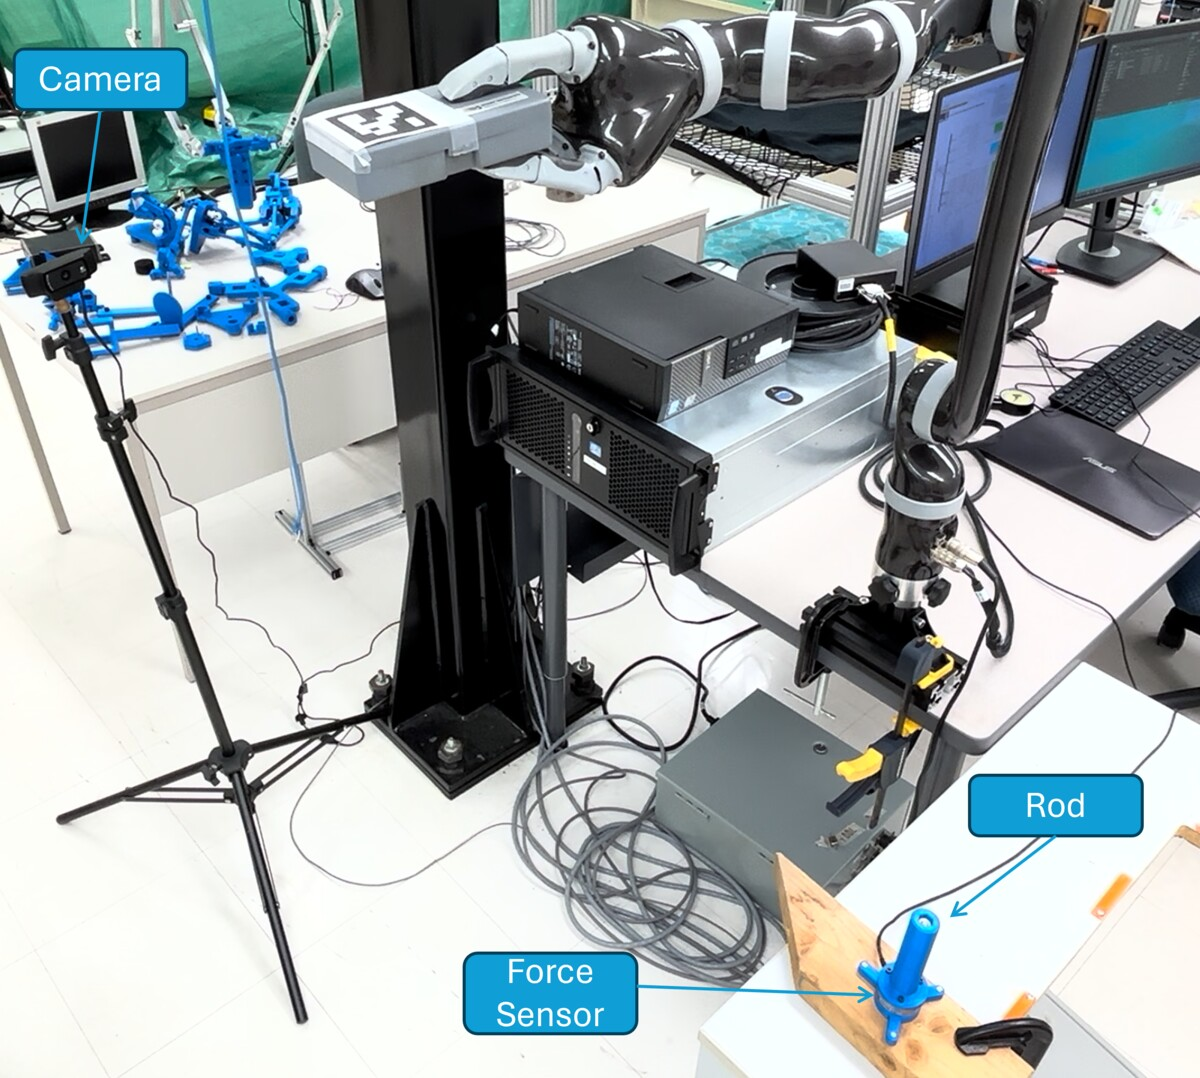
\includegraphics[width=5.1cm]{Figure7.jpg}};
  \node[paneltitle] at (6.0,4.85) {(b) MuJoCo sequence};
  \node[anchor=south west,inner sep=0] at (6.0,.95)
    {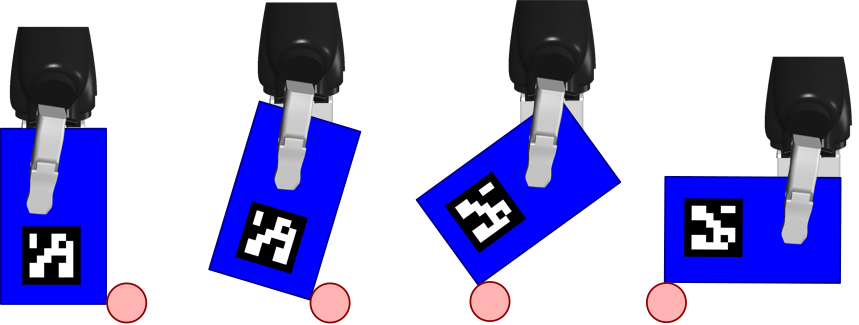
\includegraphics[width=8.4cm]{Figure6.png}};
  \foreach \x/\stage in {6.84/1,8.87/2,11.18/3,13.59/4} {
    \draw[motion,line width=1.1pt] (\x,3.95) -- ++(.385,0);
    \node[anchor=north] at (\x+.15,.85) {Stage \stage};
  }
  \node[anchor=west] at (6.0,.1) {Parallel arrows: fixed wrist orientation};
\end{tikzpicture}

\vspace{2mm}
\begin{tikzpicture}[paperfigure]
  \path[use as bounding box] (0,-.55) rectangle (15.3,5.1);
  \node[paneltitle] at (0,4.92) {(c) Hardware contact region};
  % Figure8.jpg is 3033 by 1819 pixels. Its three bottom frames
  % have equal widths. Identical lower-right regions are shown at the same scale.
  \foreach \x/\sx/\stage in {
    0/-5.5/{Approach / contact},
    5.3/-15.61/{Intermediate},
    10.6/-25.72/{Final}}
  {
    \begin{scope}[shift={(\x,0)}]
      \clip (0,0) rectangle (4.61,4.595);
      \node[anchor=south west,inner sep=0] at (\sx,0)
        {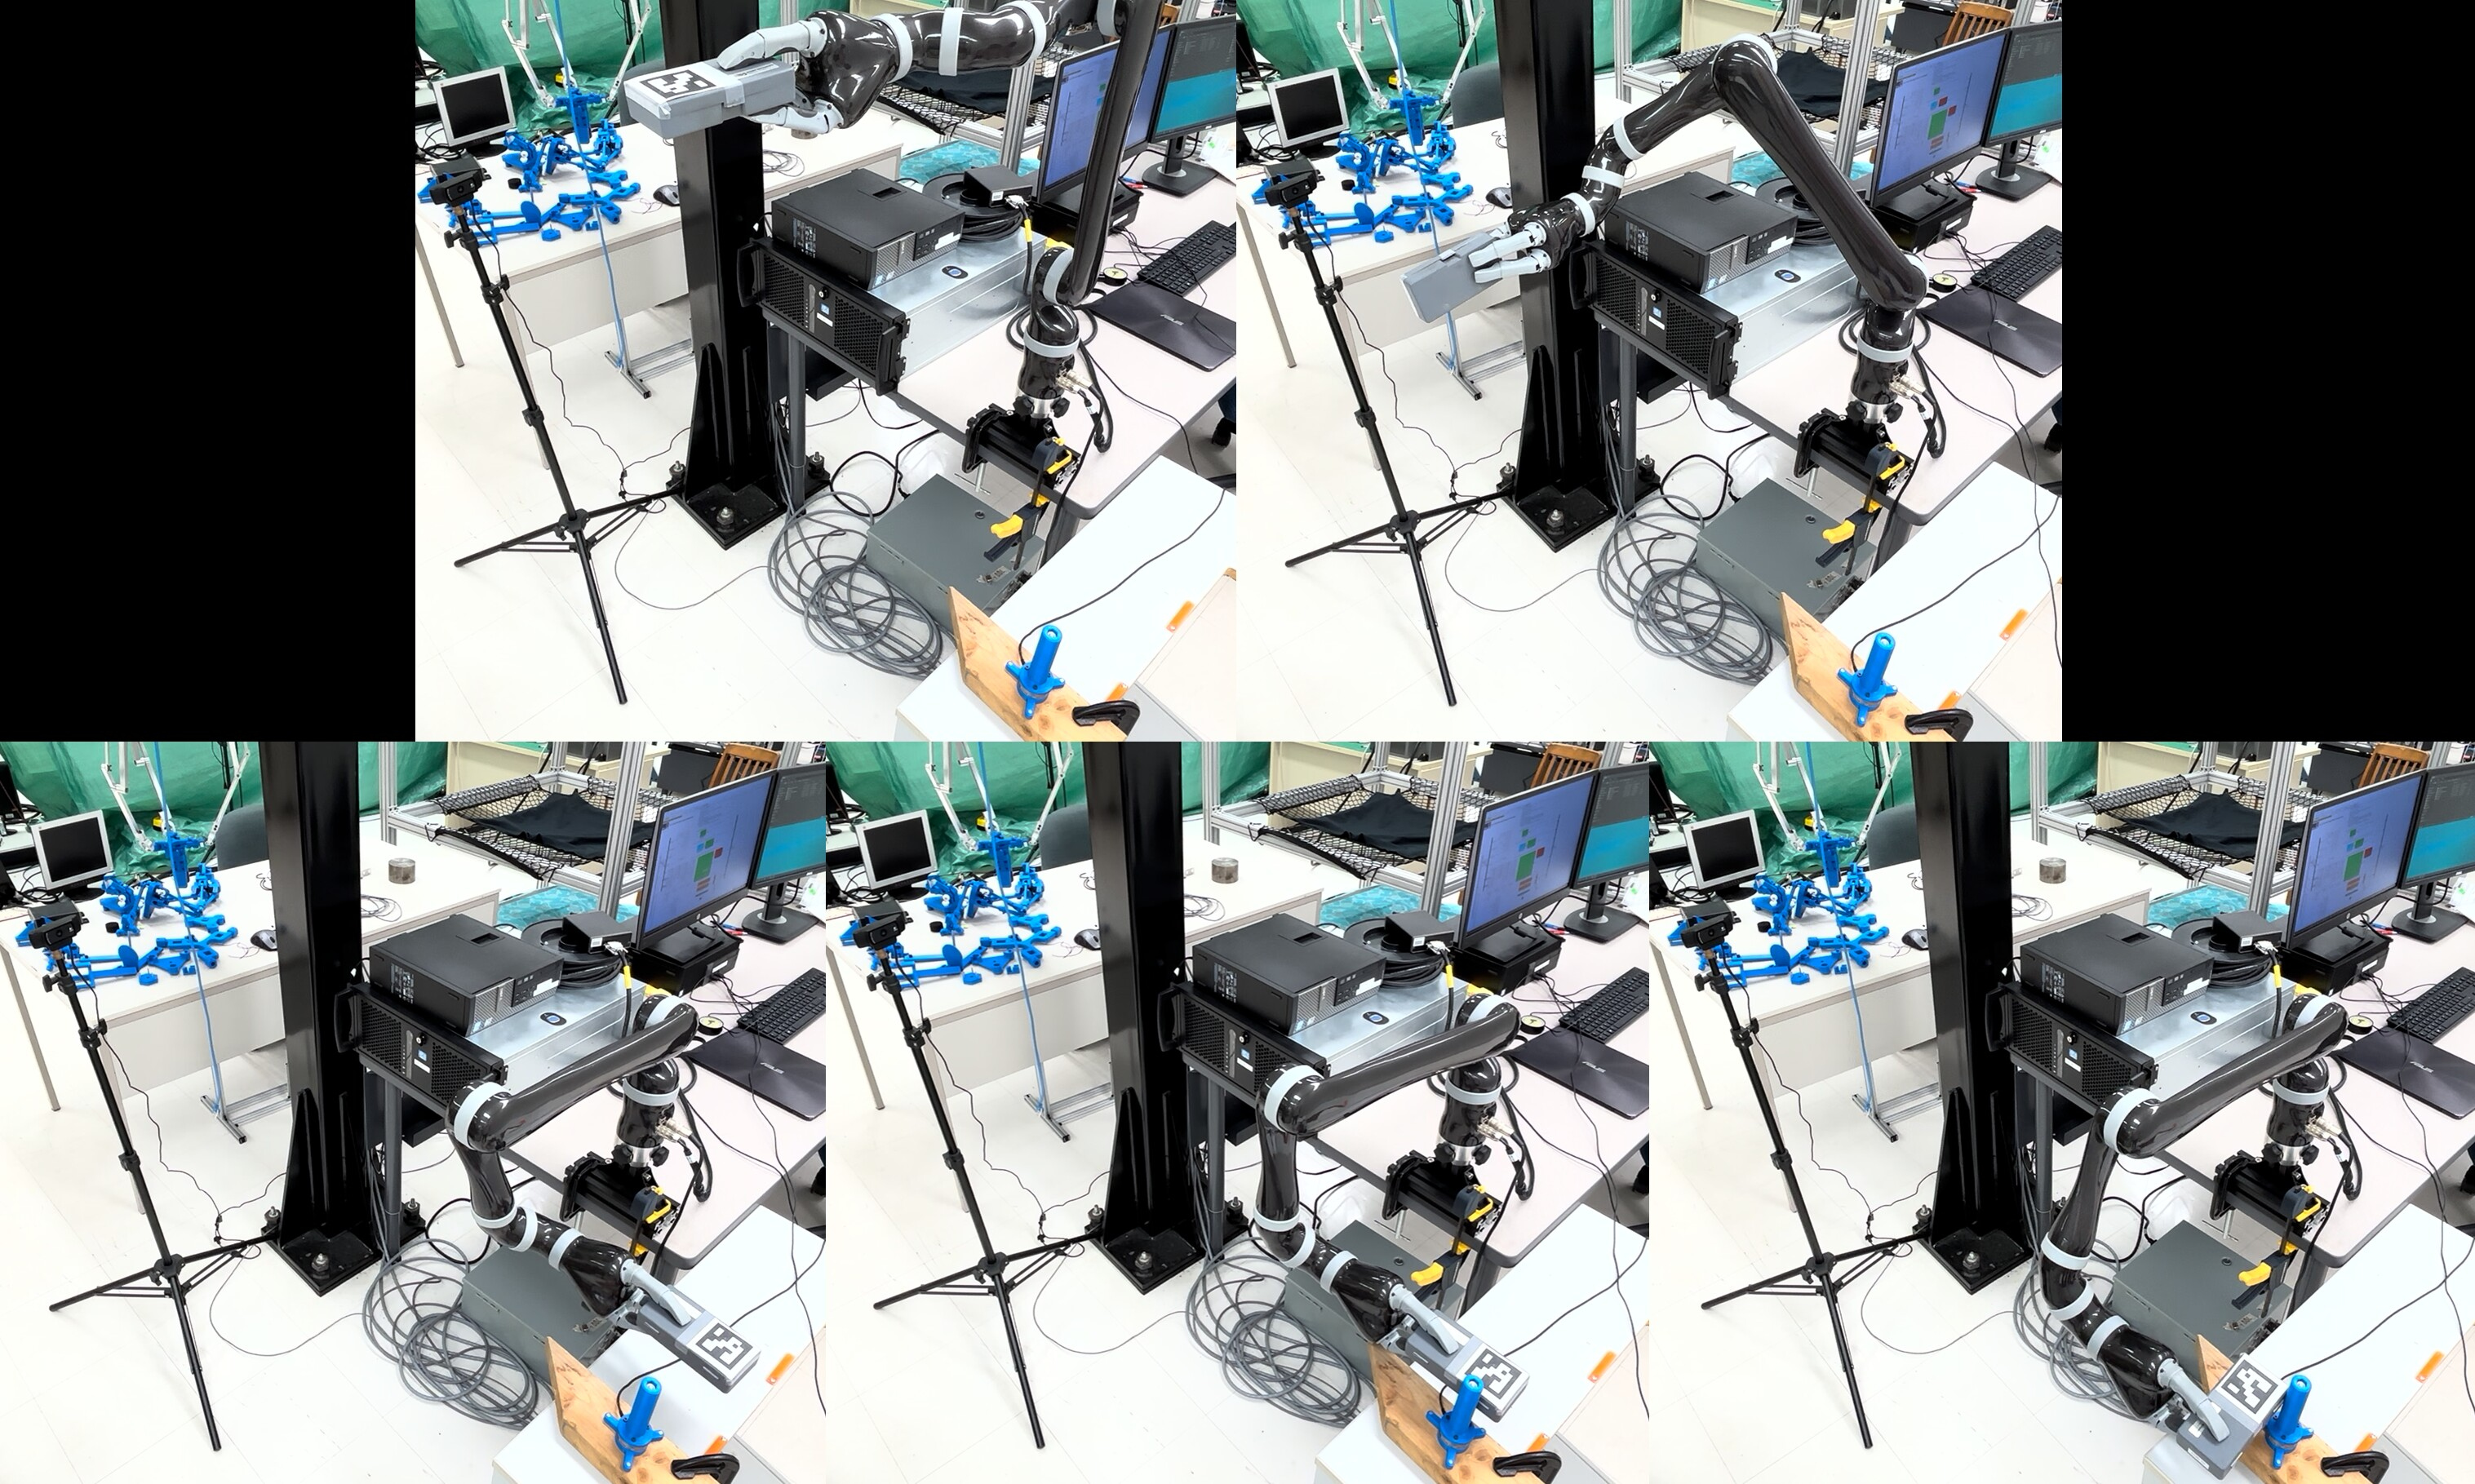
\includegraphics[width=30.33cm]{Figure8.jpg}};
    \end{scope}
    \node[anchor=north,text width=4.61cm,align=center] at (\x+2.305,-.1) {\stage};
  }
\end{tikzpicture}
\caption{Original setup and MuJoCo sequence, with three enlarged hardware contact-region crops in their original order. Stage labels carry no measured timestamps or angles.}
\label{fig:experiment_setup}
\end{figure}


\begin{table}[htbp]
    \centering
    \renewcommand{\arraystretch}{1.1}
    \begin{tabular}{ccc}
        \hline
        Initial $\rightarrow$ target ($^{\circ}$) & Simulation error ($^{\circ}$) & Hardware MAE ($^{\circ}$, $n=5$) \\
        \hline
        $0\rightarrow90$ & 0.2 & 3.6 \\
        $90\rightarrow180$ & 0.1 & 4.1 \\
        $-90\rightarrow0$ & 0.3 & 7.5 \\
        $180\rightarrow0$ & 0.2 & 4.9 \\
        \hline
    \end{tabular}
    \caption{Absolute final-angle errors of the turn: one simulation run and five hardware trials per configuration.}
    \label{tab:results}
\end{table}

The hardware mean absolute errors were $3.6^{\circ}$--$7.5^{\circ}$ (\tabref{tab:results}). Only these means were retained; signed errors, trial spread, pad dimensions, and grasp drift are unavailable. The trials therefore demonstrate the turn primitive, including its vertex-contact case, but cannot test the sign or magnitude of the under-rotation predicted by Proposition~\ref{prop:slip}.

\subsection{Shifts and complete sequences in simulation}
\label{sec:exp_tworod}

\paragraph{Configuration and predictions.}
The simulations use an $80\times30$ mm rectangular plate grasped at its centre, rods of radius $R=5$ mm, and the request $\Delta=\pi/2$, $\mathbf d=(5,20)$ mm. Then $\mathbf d_0=(20,-5)$ mm, the trailing vertex is $(-40,15)$ mm, and the weights are $\alpha_a\simeq0.24$ for the top edge and $\alpha_b\simeq0.97$ for the left edge. The meeting point $\mathbf x=(-36,9)$ mm ($\lambda\simeq37.1$ mm) gives rod centres $(-36,20)$ and $(-45,9)$ mm, spacing $D\simeq14.2$ mm, and $K_{\mathrm{sh}}\simeq11.4$ mm/rad. After the shift, the top rod has lever arm $\ell=16.0$ mm and drives the quarter turn, while the left rod's lever arm is $-4$ mm and its contact separates. Sections~\ref{sec:method} and~\ref{sec:turn} then predict the following. A placement error $e$ makes the plate tilt toward $e/K_{\mathrm{sh}}$, that is $5.0^{\circ}$ per millimetre, but by \eqref{eq:relax_end} a shift of $\|\mathbf d_0\|=20.6$ mm from an untilted start reaches only $32\%$ of it, $1.59^{\circ}$ per millimetre; for the stiffer placement $\lambda=30$ mm ($K_{\mathrm{sh}}=18.5$ mm/rad), it reaches $74\%$, $2.28^{\circ}$ per millimetre. A pad with limit-surface length $\rho$ (in millimetres) makes the turn under-rotate by $0.35\rho^2$ degrees, with a grasp drift of $0.098\rho^2$ mm toward the top edge.

\paragraph{Model.}
The simulations use MuJoCo 3.14 \cite{todorov2012mujoco}. The plate is 5 mm thick, has a mass of 0.2 kg, and touches only the pads and the rods, with gravity off. The gripper translates on two prescribed slide joints with its orientation locked, and two spherical pads of radius 1 mm pinch the plate with a constant force of 5 N each. Each pad is a single elliptic-cone contact with torsional friction, which gives the ellipsoidal limit surface of Section~\ref{sec:slip} with $\rho$ equal to the ratio of torsional to sliding friction; $\rho=2$ mm unless varied, which corresponds to a uniformly loaded disk pad of radius 3 mm. The rods have radius 5 mm and spin on undamped hinges. They are frictionless except in the comparison of free and fixed rods below: with rod friction, the solver transmitted a spurious tangential force of about 0.2--0.3 N through a free rod, which made runs with small rod loads depend on the time step, whereas by Section~\ref{sec:freerod} a free rod's wrench does not depend on its friction, which that comparison checks. Shifts run at 5 mm/s and turns at $10^{\circ}$/s with a time step of 1 ms. Of the 367 runs, 17 repeat a case at half or quarter time step and 11 at half speed; these repeats changed final angles by at most $0.04^{\circ}$. Holding the plate still against the rods for the 9 s of a turn moved it by $0.02^{\circ}$ and 0.03 mm, which bounds the solver's creep.

\paragraph{Shift.}
With the rods at the nominal placement, we offset the initial grasp across the drag line so that $e\in\{0,\pm0.5,\pm1\}$ mm and ran the shift alone. The endpoint tilt had the sign of $e$ and was linear in it, with slopes of $1.589^{\circ}$ and $2.267^{\circ}$ per millimetre for $\lambda=37.1$ and 30 mm (residuals below $0.01^{\circ}$), against $1.59^{\circ}$ and $2.28^{\circ}$ from \eqref{eq:relax_end} and asymptotes of $5.03^{\circ}$ and $3.10^{\circ}$, and along the shift it followed the solution of \eqref{eq:relax} to within $0.02^{\circ}$ (\figref{fig:sim_shift}). Halving the shift speed changed the endpoints by less than $0.01^{\circ}$, so the tilt is set by the distance travelled rather than by time, and a 3 s hold after the shift changed them by less than $0.04^{\circ}$. For a shift pushed straight into the top edge, with the rods offset by 0.5 mm along it, a single rod let the plate turn by $2.76^{\circ}$ and move by 0.48 mm over the 10 mm shift, whereas two rods straddling the grasp line held it within $0.003^{\circ}$ and 0.02 mm, as Section~\ref{sec:minimal} predicts.

\begin{figure}[htbp]
\centering
% Written by python -m simulation figures from results/simulation.json; do not edit by hand.
\begin{tikzpicture}[paperfigure]
\path[use as bounding box] (0,-0.6) rectangle (15.6,6.0);
\draw[black!12,line width=.3pt] (1.300,1.657) -- (7.100,1.657);
\draw[black!12,line width=.3pt] (1.300,2.479) -- (7.100,2.479);
\draw[black!12,line width=.3pt] (1.300,3.300) -- (7.100,3.300);
\draw[black!12,line width=.3pt] (1.300,4.121) -- (7.100,4.121);
\draw[black!12,line width=.3pt] (1.300,4.943) -- (7.100,4.943);
\draw[black!35,line width=.4pt] (1.300,3.300) -- (7.100,3.300);
\draw[black!35,line width=.4pt] (4.200,1.000) -- (4.200,5.600);
\draw[black!60,line width=.4pt] (1.300,1.000) rectangle (7.100,5.600);
\draw[black!60,line width=.4pt] (1.678,1.000) -- ++(0,.08) node[below=3pt,black!80] {$-1$};
\draw[black!60,line width=.4pt] (2.939,1.000) -- ++(0,.08) node[below=3pt,black!80] {$-0.5$};
\draw[black!60,line width=.4pt] (4.200,1.000) -- ++(0,.08) node[below=3pt,black!80] {$0$};
\draw[black!60,line width=.4pt] (5.461,1.000) -- ++(0,.08) node[below=3pt,black!80] {$0.5$};
\draw[black!60,line width=.4pt] (6.722,1.000) -- ++(0,.08) node[below=3pt,black!80] {$1$};
\draw[black!60,line width=.4pt] (1.300,1.657) -- ++(.08,0) node[left=3pt,black!80] {$-4$};
\draw[black!60,line width=.4pt] (1.300,2.479) -- ++(.08,0) node[left=3pt,black!80] {$-2$};
\draw[black!60,line width=.4pt] (1.300,3.300) -- ++(.08,0) node[left=3pt,black!80] {$0$};
\draw[black!60,line width=.4pt] (1.300,4.121) -- ++(.08,0) node[left=3pt,black!80] {$2$};
\draw[black!60,line width=.4pt] (1.300,4.943) -- ++(.08,0) node[left=3pt,black!80] {$4$};
\node[below=14pt] at (4.200,1.000) {offset $e$ (mm)};
\node[rotate=90,above=18pt] at (1.300,3.300) {endpoint tilt ($^{\circ}$)};
\draw[objectblue,densely dashed,line width=.6pt] (1.426,1.029) -- (6.974,5.571);
\draw[objectblue,line width=.8pt] (1.426,2.580) -- (6.974,4.020);
\filldraw[fill=objectblue,draw=white,line width=.4pt] (6.722,3.955) circle[radius=2.1pt];
\filldraw[fill=objectblue,draw=white,line width=.4pt] (5.461,3.625) circle[radius=2.1pt];
\filldraw[fill=objectblue,draw=white,line width=.4pt] (4.200,3.297) circle[radius=2.1pt];
\filldraw[fill=objectblue,draw=white,line width=.4pt] (2.939,2.972) circle[radius=2.1pt];
\filldraw[fill=objectblue,draw=white,line width=.4pt] (1.678,2.650) circle[radius=2.1pt];
\draw[forceorange,densely dashed,line width=.6pt] (1.426,1.901) -- (6.974,4.699);
\draw[forceorange,line width=.8pt] (1.426,2.271) -- (6.974,4.329);
\filldraw[fill=forceorange,draw=white,line width=.4pt] (6.722,4.236) ++(-1.9pt,-1.9pt) rectangle ++(3.8pt,3.8pt);
\filldraw[fill=forceorange,draw=white,line width=.4pt] (5.461,3.766) ++(-1.9pt,-1.9pt) rectangle ++(3.8pt,3.8pt);
\filldraw[fill=forceorange,draw=white,line width=.4pt] (4.200,3.299) ++(-1.9pt,-1.9pt) rectangle ++(3.8pt,3.8pt);
\filldraw[fill=forceorange,draw=white,line width=.4pt] (2.939,2.835) ++(-1.9pt,-1.9pt) rectangle ++(3.8pt,3.8pt);
\filldraw[fill=forceorange,draw=white,line width=.4pt] (1.678,2.375) ++(-1.9pt,-1.9pt) rectangle ++(3.8pt,3.8pt);
\node[anchor=south west,font=\small\bfseries] at (1.300,5.600) {(a)};
\filldraw[fill=objectblue,draw=white,line width=.4pt] (1.678,5.189) circle[radius=2.1pt];
\node[anchor=west,font=\scriptsize] at (1.880,5.189) {$\lambda=37.1$ mm};
\filldraw[fill=forceorange,draw=white,line width=.4pt] (1.678,4.820) ++(-1.9pt,-1.9pt) rectangle ++(3.8pt,3.8pt);
\node[anchor=west,font=\scriptsize] at (1.880,4.820) {$\lambda=30$ mm};
\draw[black!12,line width=.3pt] (9.200,1.000) -- (15.000,1.000);
\draw[black!12,line width=.3pt] (9.200,1.767) -- (15.000,1.767);
\draw[black!12,line width=.3pt] (9.200,2.533) -- (15.000,2.533);
\draw[black!12,line width=.3pt] (9.200,3.300) -- (15.000,3.300);
\draw[black!12,line width=.3pt] (9.200,4.067) -- (15.000,4.067);
\draw[black!12,line width=.3pt] (9.200,4.833) -- (15.000,4.833);
\draw[black!60,line width=.4pt] (9.200,1.000) rectangle (15.000,5.600);
\draw[black!60,line width=.4pt] (9.200,1.000) -- ++(0,.08) node[below=3pt,black!80] {$0$};
\draw[black!60,line width=.4pt] (10.581,1.000) -- ++(0,.08) node[below=3pt,black!80] {$5$};
\draw[black!60,line width=.4pt] (11.962,1.000) -- ++(0,.08) node[below=3pt,black!80] {$10$};
\draw[black!60,line width=.4pt] (13.343,1.000) -- ++(0,.08) node[below=3pt,black!80] {$15$};
\draw[black!60,line width=.4pt] (14.724,1.000) -- ++(0,.08) node[below=3pt,black!80] {$20$};
\draw[black!60,line width=.4pt] (9.200,1.000) -- ++(.08,0) node[left=3pt,black!80] {$0$};
\draw[black!60,line width=.4pt] (9.200,1.767) -- ++(.08,0) node[left=3pt,black!80] {$1$};
\draw[black!60,line width=.4pt] (9.200,2.533) -- ++(.08,0) node[left=3pt,black!80] {$2$};
\draw[black!60,line width=.4pt] (9.200,3.300) -- ++(.08,0) node[left=3pt,black!80] {$3$};
\draw[black!60,line width=.4pt] (9.200,4.067) -- ++(.08,0) node[left=3pt,black!80] {$4$};
\draw[black!60,line width=.4pt] (9.200,4.833) -- ++(.08,0) node[left=3pt,black!80] {$5$};
\node[below=14pt] at (12.100,1.000) {grasp travel $s$ (mm)};
\node[rotate=90,above=18pt] at (9.200,3.300) {tilt ($^{\circ}$)};
\draw[objectblue,densely dashed,line width=.6pt] (9.200,4.854) -- (15.000,4.854);
\draw[objectblue,line width=.8pt] (9.200,1.000) -- (9.314,1.013) -- (9.428,1.027) -- (9.542,1.041) -- (9.657,1.055) -- (9.771,1.069) -- (9.885,1.084) -- (9.999,1.099) -- (10.113,1.114) -- (10.227,1.129) -- (10.342,1.145) -- (10.456,1.161) -- (10.570,1.178) -- (10.684,1.195) -- (10.798,1.212) -- (10.912,1.230) -- (11.027,1.248) -- (11.141,1.266) -- (11.255,1.285) -- (11.369,1.304) -- (11.483,1.324) -- (11.597,1.344) -- (11.712,1.364) -- (11.826,1.386) -- (11.940,1.407) -- (12.054,1.429) -- (12.168,1.452) -- (12.282,1.475) -- (12.397,1.499) -- (12.511,1.523) -- (12.625,1.548) -- (12.739,1.574) -- (12.853,1.600) -- (12.967,1.628) -- (13.081,1.655) -- (13.196,1.684) -- (13.310,1.713) -- (13.424,1.743) -- (13.538,1.774) -- (13.652,1.806) -- (13.766,1.839) -- (13.881,1.873) -- (13.995,1.907) -- (14.109,1.943) -- (14.223,1.980) -- (14.337,2.018) -- (14.451,2.057) -- (14.566,2.098) -- (14.680,2.139) -- (14.794,2.182);
\filldraw[fill=objectblue,draw=white,line width=.4pt] (9.476,1.026) circle[radius=2.1pt];
\filldraw[fill=objectblue,draw=white,line width=.4pt] (10.029,1.096) circle[radius=2.1pt];
\filldraw[fill=objectblue,draw=white,line width=.4pt] (10.581,1.173) circle[radius=2.1pt];
\filldraw[fill=objectblue,draw=white,line width=.4pt] (11.133,1.258) circle[radius=2.1pt];
\filldraw[fill=objectblue,draw=white,line width=.4pt] (11.686,1.354) circle[radius=2.1pt];
\filldraw[fill=objectblue,draw=white,line width=.4pt] (12.238,1.460) circle[radius=2.1pt];
\filldraw[fill=objectblue,draw=white,line width=.4pt] (12.791,1.581) circle[radius=2.1pt];
\filldraw[fill=objectblue,draw=white,line width=.4pt] (13.343,1.718) circle[radius=2.1pt];
\filldraw[fill=objectblue,draw=white,line width=.4pt] (13.895,1.874) circle[radius=2.1pt];
\filldraw[fill=objectblue,draw=white,line width=.4pt] (14.448,2.055) circle[radius=2.1pt];
\draw[forceorange,densely dashed,line width=.6pt] (9.200,3.374) -- (15.000,3.374);
\draw[forceorange,line width=.8pt] (9.200,1.000) -- (9.314,1.020) -- (9.428,1.041) -- (9.542,1.062) -- (9.657,1.084) -- (9.771,1.105) -- (9.885,1.128) -- (9.999,1.151) -- (10.113,1.174) -- (10.227,1.198) -- (10.342,1.222) -- (10.456,1.247) -- (10.570,1.272) -- (10.684,1.298) -- (10.798,1.324) -- (10.912,1.351) -- (11.027,1.378) -- (11.141,1.406) -- (11.255,1.435) -- (11.369,1.464) -- (11.483,1.494) -- (11.597,1.525) -- (11.712,1.556) -- (11.826,1.588) -- (11.940,1.620) -- (12.054,1.654) -- (12.168,1.688) -- (12.282,1.723) -- (12.397,1.758) -- (12.511,1.795) -- (12.625,1.832) -- (12.739,1.870) -- (12.853,1.909) -- (12.967,1.949) -- (13.081,1.989) -- (13.196,2.031) -- (13.310,2.073) -- (13.424,2.116) -- (13.538,2.161) -- (13.652,2.206) -- (13.766,2.252) -- (13.881,2.299) -- (13.995,2.346) -- (14.109,2.395) -- (14.223,2.444) -- (14.337,2.494) -- (14.451,2.545) -- (14.566,2.596) -- (14.680,2.648) -- (14.794,2.700);
\filldraw[fill=forceorange,draw=white,line width=.4pt] (9.476,1.042) ++(-1.9pt,-1.9pt) rectangle ++(3.8pt,3.8pt);
\filldraw[fill=forceorange,draw=white,line width=.4pt] (10.029,1.148) ++(-1.9pt,-1.9pt) rectangle ++(3.8pt,3.8pt);
\filldraw[fill=forceorange,draw=white,line width=.4pt] (10.581,1.266) ++(-1.9pt,-1.9pt) rectangle ++(3.8pt,3.8pt);
\filldraw[fill=forceorange,draw=white,line width=.4pt] (11.133,1.397) ++(-1.9pt,-1.9pt) rectangle ++(3.8pt,3.8pt);
\filldraw[fill=forceorange,draw=white,line width=.4pt] (11.686,1.542) ++(-1.9pt,-1.9pt) rectangle ++(3.8pt,3.8pt);
\filldraw[fill=forceorange,draw=white,line width=.4pt] (12.238,1.703) ++(-1.9pt,-1.9pt) rectangle ++(3.8pt,3.8pt);
\filldraw[fill=forceorange,draw=white,line width=.4pt] (12.791,1.883) ++(-1.9pt,-1.9pt) rectangle ++(3.8pt,3.8pt);
\filldraw[fill=forceorange,draw=white,line width=.4pt] (13.343,2.083) ++(-1.9pt,-1.9pt) rectangle ++(3.8pt,3.8pt);
\filldraw[fill=forceorange,draw=white,line width=.4pt] (13.895,2.304) ++(-1.9pt,-1.9pt) rectangle ++(3.8pt,3.8pt);
\filldraw[fill=forceorange,draw=white,line width=.4pt] (14.448,2.545) ++(-1.9pt,-1.9pt) rectangle ++(3.8pt,3.8pt);
\node[anchor=south west,font=\small\bfseries] at (9.200,5.600) {(b)};
\node[anchor=south east,objectblue!90!black,font=\scriptsize] at (14.890,4.946) {$e/K_{\mathrm{sh}}$, $\lambda=37.1$};
\node[anchor=south east,forceorange!90!black,font=\scriptsize] at (14.890,3.466) {$e/K_{\mathrm{sh}}$, $\lambda=30$};
\filldraw[fill=black!60,draw=white] (3.2,-0.35) circle[radius=2.1pt]; \node[anchor=west] at (3.35,-0.35) {simulation};
\draw[black!70,line width=.8pt] (5.6,-0.35) -- (6.1,-0.35); \node[anchor=west] at (6.15,-0.35) {prediction, Eqs.~(\ref{eq:relax})--(\ref{eq:relax_end})};
\draw[black!70,densely dashed,line width=.6pt] (10.4,-0.35) -- (10.9,-0.35); \node[anchor=west] at (10.95,-0.35) {asymptote $e/K_{\mathrm{sh}}$};
\end{tikzpicture}
\caption{Shift tilt in simulation for the placements $\lambda=37.1$ and 30 mm. (a)~Tilt at the end of the shift against the grasp offset $e$, with the finite-shift prediction \eqref{eq:relax_end} (solid) and the asymptote $e/K_{\mathrm{sh}}$ of Proposition~\ref{prop:stiffness} (dashed). (b)~Tilt along the shift for $e=1$ mm, with the solution of \eqref{eq:relax}: the plate approaches $e/K_{\mathrm{sh}}$ at the predicted rate and does not reach it.}
\label{fig:sim_shift}
\end{figure}


\paragraph{Turn.}
\tabref{tab:sim_turn} and \figref{fig:sim_turn} compare the turn alone, about one rod on the top edge, with Proposition~\ref{prop:slip} and with the same limit-surface model integrated without linearization. The simulated under-rotation exceeded the integrated model by $0.05^{\circ}$--$0.09^{\circ}$ in every case but $\ell=8$ mm ($0.17^{\circ}$), a small positive offset a few times the creep floor. The first-order estimate agrees with both to within that offset up to $\rho/\ell=0.125$ and overstates the slip beyond, by $0.24^{\circ}$ at $\rho/\ell=0.19$ and $1.55^{\circ}$ at $\rho/\ell=0.31$ in the integrated model. The grasp drifted toward the contact along the edge normal as predicted, with a component along the edge below 0.03 mm. The corner contact ($\ell=20$ mm), the case run on hardware, under-rotated by $0.96^{\circ}$ against $0.90^{\circ}$ predicted.

% Written by python -m simulation tables from results/simulation.json; do not edit by hand.
\begin{table}[htbp]
    \centering
    \renewcommand{\arraystretch}{1.1}
    \begin{tabular}{cccccccc}
        \hline
        $\rho$ (mm) & $\ell$ (mm) & $\rho/\ell$ & \multicolumn{3}{c}{Under-rotation ($^{\circ}$)} & \multicolumn{2}{c}{Grasp drift (mm)} \\
        & & & first order & integrated & simulated & first order & simulated \\
        \hline
        0.5 & 16 & 0.031 & 0.09 & 0.09 & 0.14 & 0.025 & 0.039 \\
        1 & 16 & 0.063 & 0.35 & 0.35 & 0.41 & 0.098 & 0.112 \\
        2 & 20 & 0.100 & 0.90 & 0.88 & 0.96 & 0.314 & 0.326 \\
        2 & 16 & 0.125 & 1.41 & 1.36 & 1.44 & 0.393 & 0.402 \\
        2 & 12 & 0.167 & 2.50 & 2.32 & 2.40 & 0.524 & 0.509 \\
        3 & 16 & 0.188 & 3.16 & 2.92 & 3.00 & 0.884 & 0.850 \\
        2 & 8 & 0.250 & 5.63 & 4.62 & 4.78 & 0.785 & 0.710 \\
        4 & 16 & 0.250 & 5.63 & 4.92 & 5.00 & 1.571 & 1.440 \\
        5 & 16 & 0.313 & 8.79 & 7.23 & 7.31 & 2.454 & 2.146 \\
        \hline
    \end{tabular}
    \caption{Turn slip in simulation for a $90^{\circ}$ turn about one free rod. First order: the estimates $\Delta\rho^2/\ell^2$ and $|\Delta|\rho^2/\ell$ of Proposition~\ref{prop:slip}; integrated: the same limit-surface model without linearization. Drift is measured along the contact normal. The row $\ell=20$ mm is the corner contact.}
    \label{tab:sim_turn}
\end{table}


\begin{figure}[htbp]
\centering
% Written by python -m simulation figures from results/simulation.json; do not edit by hand.
\begin{tikzpicture}[paperfigure]
\path[use as bounding box] (-0.1,0.0) rectangle (10.6,6.6);
\draw[black!12,line width=.3pt] (1.300,1.000) -- (10.300,1.000);
\draw[black!12,line width=.3pt] (1.300,2.149) -- (10.300,2.149);
\draw[black!12,line width=.3pt] (1.300,3.298) -- (10.300,3.298);
\draw[black!12,line width=.3pt] (1.300,4.447) -- (10.300,4.447);
\draw[black!12,line width=.3pt] (1.300,5.596) -- (10.300,5.596);
\draw[black!60,line width=.4pt] (1.300,1.000) rectangle (10.300,6.400);
\draw[black!60,line width=.4pt] (1.300,1.000) -- ++(0,.08) node[below=3pt,black!80] {$0$};
\draw[black!60,line width=.4pt] (3.100,1.000) -- ++(0,.08) node[below=3pt,black!80] {$0.02$};
\draw[black!60,line width=.4pt] (4.900,1.000) -- ++(0,.08) node[below=3pt,black!80] {$0.04$};
\draw[black!60,line width=.4pt] (6.700,1.000) -- ++(0,.08) node[below=3pt,black!80] {$0.06$};
\draw[black!60,line width=.4pt] (8.500,1.000) -- ++(0,.08) node[below=3pt,black!80] {$0.08$};
\draw[black!60,line width=.4pt] (10.300,1.000) -- ++(0,.08) node[below=3pt,black!80] {$0.1$};
\draw[black!60,line width=.4pt] (1.300,1.000) -- ++(.08,0) node[left=3pt,black!80] {$0$};
\draw[black!60,line width=.4pt] (1.300,2.149) -- ++(.08,0) node[left=3pt,black!80] {$2$};
\draw[black!60,line width=.4pt] (1.300,3.298) -- ++(.08,0) node[left=3pt,black!80] {$4$};
\draw[black!60,line width=.4pt] (1.300,4.447) -- ++(.08,0) node[left=3pt,black!80] {$6$};
\draw[black!60,line width=.4pt] (1.300,5.596) -- ++(.08,0) node[left=3pt,black!80] {$8$};
\node[below=14pt] at (5.800,1.000) {$\rho^2/\ell^2$};
\node[rotate=90,above=18pt] at (1.300,3.700) {under-rotation ($^{\circ}$)};
\draw[black!75,line width=.6pt] (1.300,1.000) -- (10.300,6.170);
\draw[objectblue,line width=.8pt] (1.300,1.000) -- (1.314,1.008) -- (1.356,1.032) -- (1.427,1.072) -- (1.525,1.128) -- (1.652,1.200) -- (1.806,1.287) -- (1.989,1.389) -- (2.200,1.505) -- (2.439,1.635) -- (2.706,1.778) -- (3.002,1.935) -- (3.325,2.104) -- (3.677,2.284) -- (4.056,2.476) -- (4.464,2.679) -- (4.900,2.891) -- (5.364,3.113) -- (5.856,3.343) -- (6.377,3.582) -- (6.925,3.828) -- (7.502,4.082) -- (8.106,4.342) -- (8.739,4.608) -- (9.400,4.879) -- (10.089,5.156);
\draw[forceorange,line width=.8pt] (7.700,3.926) -- (6.925,3.652) -- (6.283,3.409) -- (5.744,3.195) -- (5.289,3.006) -- (4.900,2.838) -- (4.565,2.689) -- (4.275,2.556) -- (4.022,2.438) -- (3.800,2.331) -- (3.604,2.236) -- (3.430,2.150) -- (3.275,2.072) -- (3.137,2.002) -- (3.012,1.938) -- (2.900,1.880) -- (2.798,1.827) -- (2.706,1.778) -- (2.622,1.734) -- (2.546,1.693) -- (2.476,1.656) -- (2.411,1.621) -- (2.352,1.589) -- (2.297,1.559) -- (2.247,1.532) -- (2.200,1.506);
\filldraw[fill=forceorange,draw=white,line width=.4pt] (6.925,3.747) ++(-1.9pt,-1.9pt) rectangle ++(3.8pt,3.8pt);
\filldraw[fill=forceorange,draw=white,line width=.4pt] (3.800,2.380) ++(-1.9pt,-1.9pt) rectangle ++(3.8pt,3.8pt);
\filldraw[fill=forceorange,draw=white,line width=.4pt] (2.706,1.828) ++(-1.9pt,-1.9pt) rectangle ++(3.8pt,3.8pt);
\filldraw[fill=forceorange,draw=white,line width=.4pt] (2.200,1.549) ++(-1.9pt,-1.9pt) rectangle ++(3.8pt,3.8pt);
\filldraw[fill=objectblue,draw=white,line width=.4pt] (1.388,1.082) circle[radius=2.1pt];
\filldraw[fill=objectblue,draw=white,line width=.4pt] (1.652,1.234) circle[radius=2.1pt];
\filldraw[fill=objectblue,draw=white,line width=.4pt] (2.706,1.828) circle[radius=2.1pt];
\filldraw[fill=objectblue,draw=white,line width=.4pt] (4.464,2.723) circle[radius=2.1pt];
\filldraw[fill=objectblue,draw=white,line width=.4pt] (6.925,3.870) circle[radius=2.1pt];
\filldraw[fill=objectblue,draw=white,line width=.4pt] (10.089,5.200) circle[radius=2.1pt];
\node[anchor=south east,black!80,font=\scriptsize] at (7.420,4.964) {first order, $\Delta\rho^2/\ell^2$};
\filldraw[fill=objectblue,draw=white,line width=.4pt] (1.750,5.940) circle[radius=2.1pt];
\node[anchor=west,font=\scriptsize] at (1.975,5.940) {$\rho$ sweep, $\ell=16$ mm};
\filldraw[fill=forceorange,draw=white,line width=.4pt] (1.750,5.481) ++(-1.9pt,-1.9pt) rectangle ++(3.8pt,3.8pt);
\node[anchor=west,font=\scriptsize] at (1.975,5.481) {$\ell$ sweep, $\rho=2$ mm};
\node[anchor=south east,black!70,font=\scriptsize] at (10.210,1.201) {markers: simulation; coloured lines: integrated model};
\end{tikzpicture}
\caption{Turn slip in simulation for a $90^{\circ}$ turn about one free rod: the $\rho$ sweep at $\ell=16$ mm (circles) and the $\ell$ sweep at $\rho=2$ mm (squares), with the first-order estimate of Proposition~\ref{prop:slip} (black) and the same limit-surface model integrated without linearization for each sweep (coloured).}
\label{fig:sim_turn}
\end{figure}


With the rod free, rod friction coefficients of 0, 0.5, and 1 gave under-rotations of $1.44^{\circ}$, $1.42^{\circ}$, and $1.44^{\circ}$ for $\rho=2$ mm and $\ell=16$ mm. With the rod welded, coefficients of 0.1, 0.2, and 0.3 gave $1.34^{\circ}$, $1.27^{\circ}$, and $1.21^{\circ}$, and the grasp also drifted along the edge, by up to 0.08 mm. Here $\mathbf n^T\mathbf p=10$ mm is positive, so a fixed rod's friction lengthens the effective lever arm of \eqref{eq:fixedrod} and reduces the slip. The bearing therefore does not make the turn more accurate; it makes the result independent of an unknown coefficient, which a fixed rod would make larger or smaller depending on its value and on the sign of $\mathbf n^T\mathbf p$. Welded rods with friction 0.5 and 1 produced stick-slip that did not converge with the time step and are not reported.

\paragraph{Complete sequences.}
In ten runs of the nominal sequence, with the engagement position perturbed by up to 0.3 mm, the grip retained the plate, and the final in-grasp rotation fell short of $90^{\circ}$ by $1.10^{\circ}$--$1.56^{\circ}$ (mean $1.32^{\circ}$). Each run's error was the tilt the plate had acquired by the end of the shift, between $-0.17^{\circ}$ and $0.31^{\circ}$, plus a turn under-rotation of $1.40^{\circ}\pm0.01^{\circ}$, against $1.41^{\circ}$ predicted. The final grasp lay 0.30--0.44 mm from its target toward the top edge, mostly the turn's drift of 0.40 mm (0.39 mm predicted). In every run, rod $b$'s force vanished 3 ms after the turn began and its gap opened within 14 ms, as Proposition~\ref{lem:separation} predicts. The one-edge sequence (a shift into the top edge against two rods, retreat, carry, re-approach to one rod with $\ell=35$ mm, and turn) ended $0.29^{\circ}$ and 0.18 mm from the request, as predicted, and the other rod was not touched after the retreat.

\paragraph{Sensing at first contact.}
The last experiment repeats the turn with $\ell=16$ mm under grasp uncertainty: a grasp position error uniform within $\pm2$ mm in each direction, an initial in-grasp orientation error uniform within $\pm3^{\circ}$, and Gaussian noise with a standard deviation of $1^{\circ}$ on the measured force direction. Each strategy ran the same 50 perturbations, and a second block added rod calibration errors uniform within $\pm0.5$ mm. Without sensing, the gripper moved to the planned engagement pose and orbited the planned centre. It touched the rod in every trial, but its angle error was dominated by the grasp offset along the contact normal, about $3.4^{\circ}$ per millimetre, close to the $1/\ell=3.6^{\circ}$ per millimetre by which an offset delays or advances the start of pivoting. Approaching until the rod's force sensor detected touch removed that dependence; the error then followed the initial orientation error (slope 0.96), offset by the turn slip. Using the measured force direction as well to estimate the initial orientation reduced the slope to 0.16, leaving a spread of $0.9^{\circ}$ set by the sensor noise around the same slip offset (\tabref{tab:sim_sensing}). Calibration errors raised its root-mean-square error from $1.6^{\circ}$ to $2.1^{\circ}$. No trial met the abort conditions, so these runs do not test them, and no strategy corrects the grasp position error, which left the final position 1.8 mm from the request on average with touch sensing.

% Written by python -m simulation tables from results/simulation.json; do not edit by hand.
\begin{table}[htbp]
    \centering
    \renewcommand{\arraystretch}{1.1}
    \begin{tabular}{lcccc}
        \hline
        Strategy & Mean ($^{\circ}$) & SD ($^{\circ}$) & RMS ($^{\circ}$) & Slope \\
        \hline
        Open loop & $-1.91$ & 4.10 & 4.48 & -- \\
        Touch & $-1.35$ & 1.60 & 2.08 & 0.96 \\
        Touch and direction & $-1.29$ & 0.90 & 1.57 & 0.16 \\
        \hline
        Open loop, calibration error & $-1.86$ & 4.17 & 4.53 & -- \\
        Touch, calibration error & $-1.28$ & 2.08 & 2.43 & 0.96 \\
        Touch and direction, calibration error & $-1.23$ & 1.74 & 2.11 & 0.17 \\
        \hline
    \end{tabular}
    \caption{Final in-grasp angle error of the turn under grasp uncertainty, 50 trials per row with the same perturbations in each block. Slope: regression of the error on the injected initial orientation error.}
    \label{tab:sim_sensing}
\end{table}


\section{Discussion and Conclusion}
\label{sec:discussion}
\label{sec:conclusion}

A simple gripper can gain in-grasp dexterity from its workspace rather than from more sensing, actuation, or planning, and the geometry that provides it can be designed in closed form. The method followed here has three steps: identify what passive contacts can and cannot prescribe, choose the fewest constraints that supply each missing motion, and place them by construction. For planar in-grasp manipulation, it leads to two free rods, a segment, and an arc. Because passive contacts cannot determine a motion that combines sliding and turning in the grip, a request is executed as a shift and then a turn. The shift sets the number of rods: two rods hold any admissible direction in one motion, with a closed-form stiffness, where one rod holds only finitely many directions and only indifferently. The turn needs one of them, at an edge or a vertex. The bearing makes the turn's contact wrench independent of rod friction, which yields a friction-free estimate of grasp slip, and across a vertex the second rod separates automatically when the turn begins. A quadratic equation tests whether an installed pair realizes a constructed placement. The individual ingredients are classical; what the paper contributes is a design rule small enough to apply by hand, in which no planning quantity depends on a friction coefficient or a force value. In practice, the tool is two pins on bearings, the gripper and its controller are unchanged, and the manipulation motions use no sensing, which makes the approach a candidate low-cost alternative to a regrasp station or a more dexterous hand. Hardware trials demonstrate turns, including the vertex-contact case; in simulation, shift tilts followed the predicted approach to $e/K_{\mathrm{sh}}$ to within 0.5\%, turn slip followed the first-order estimate to within $0.06^{\circ}$ for $\rho/\ell\leq0.125$, and complete sequences, including one with re-engagement, ended within the predicted slip.

The construction assumes a polygonal outline, convex or not, touched by each rod at a single point, a known interior grasp, a pinch normal to the plane, quasi-static motion, and grip settings that retain the object while allowing sliding and pivoting. The stiffness and slip results are first-order estimates. The slip, and the rate at which a shift approaches the stiffness tilt, rest on an ellipsoidal limit surface for the pad, and the slip also neglects bearing friction; all should be read as design trends rather than exact predictions. The hardware trials used a single rod, retained only mean absolute errors, and cannot test the predicted under-rotation. Fixed spacing, accessible contacts, grasp travel, clearance, and robot reach limit the usable requests; the wrist may rotate before engagement but is held during manipulation. Hardware shifts and complete sequences remain to be tested. Whether one installed pair reaches every usable grasp and orientation by chaining motions, and how to trade the number of motions against the stiffness of each, are still open. So is the extension of the same three-step method to other changes of grasp, such as flipping a part out of the plane, where the missing constraints and their minimal geometry would differ.


\FloatBarrier

\bibliographystyle{unsrtnat}
\begingroup
\small
\bibliography{refs}
\endgroup

\end{document}
